\documentclass[10pt]{article}
\usepackage[polish]{babel}
\usepackage[utf8]{inputenc}
\usepackage[T1]{fontenc}
\usepackage{amsmath}
\usepackage{amsfonts}
\usepackage{amssymb}
\usepackage[version=4]{mhchem}
\usepackage{stmaryrd}
\usepackage{graphicx}
\usepackage[export]{adjustbox}
\graphicspath{ {./images/} }
\usepackage{multirow}

\newcommand\Varangle{\mathop{{<\!\!\!\!\!\text{\small)}}\:}\nolimits}

\begin{document}
\section*{EGZAMIN MATURALNY}
\section*{W ROKU SZKOLNYM 2017/2018}
\section*{MATEMATYKA}
POZIOM ROZSZERZONY\\
FORMUŁA OD 2015\\
(,,NOWA MATURA")

ZASADY OCENIANIA ROZWIĄZAŃ ZADAŃ\\
ARKUSZ MMA-R1

\section*{Zadania zamknięte}
Punkt przyznaje się za wskazanie poprawnej odpowiedzi.\\
Zadanie 1. (0-1)

\begin{center}
\begin{tabular}{|l|l|c|}
\hline
\multicolumn{1}{|c|}{Wymagania ogólne} & \multicolumn{1}{c|}{Wymagania szczegółowe} & \begin{tabular}{c}
Poprawna \\
odpowiedź \\
\end{tabular} \\
\hline
\begin{tabular}{l}
II. Wykorzystanie \\
i interpretowanie \\
reprezentacji. \\
\end{tabular} & \begin{tabular}{l}
1. Liczby rzeczywiste. Zdajaccy oblicza potęgi \\
o wykładnikach wymiernych i stosuje prawa \\
działań na potęgach o wykładnikach wymiernych \\
(1.4). \\
\end{tabular} & A \\
\hline
\end{tabular}
\end{center}

Zadanie 2. (0-1)

\begin{center}
\begin{tabular}{|l|l|c|}
\hline
 & \begin{tabular}{l}
1. Liczby rzeczywiste. Zdający wykorzystuje \\
pojęcie wartości bezwzględnej i jej interpretację \\
geometryczną (R1.1). \\
\end{tabular} & B \\
I. Wykorzystanie & \begin{tabular}{l}
i tworzenie informacji. \\
ALBO \\
3. Równania i nierówności. Zdający rozwiązuje \\
równania i nierówności z wartością bezwzględną \\
(R3.9). \\
\end{tabular} & B \\
\hline
\end{tabular}
\end{center}

\section*{Zadanie 3. (0-1)}
II. Wykorzystanie i interpretowanie reprezentacji.

\begin{enumerate}
  \item Liczby rzeczywiste. Zdający stosuje w obliczeniach wzór na logarytm potęgi oraz wzór na zamianę podstawy logarytmu (R1.2).
\end{enumerate}

C

Zadanie 4. (0-1)\\
II. Wykorzystanie i interpretowanie reprezentacji.\\
11. Rachunek różniczkowy. Zdający oblicza granice funkcji (i granice jednostronne), korzystając z twierdzeń o działaniach na granicach i z własności funkcji ciągłych (R11.1).

Zadanie 5. (0-2)

\begin{center}
\begin{tabular}{|l|l|c|}
\hline
 & \begin{tabular}{l}
11. Rachunek różniczkowy. Zdający oblicza \\
granice funkcji (i granice jednostronne), \\
korzystając z twierdzeń o działaniach na \\
granicach i z własności funkcji ciągłych (R11.1). \\
\end{tabular} & $\mathbf{1 6 6}$ \\
\begin{tabular}{l}
II. Wykorzystanie \\
i interpretowanie \\
reprezentacji. \\
\end{tabular} & \begin{tabular}{l}
4. Funkcje. Zdajajcy odczytuje z wykresu \\
własności funkcji (dziedzinę, zbiór wartości) \\
(4.2). \\
\end{tabular} &  \\
\hline
\end{tabular}
\end{center}

\section*{Ogólne zasady oceniania zadań otwartych}
Uwaga: Akceptowane sq wszystkie odpowiedzi merytorycznie poprawne i spetniajace warunki zadania.

\section*{Zadanie 6. (0-3)}
\begin{center}
\begin{tabular}{|l|l|}
\hline
\multicolumn{1}{|c|}{Wymagania ogólne} & \multicolumn{1}{c|}{Wymagania szczegółowe} \\
\hline
\begin{tabular}{l}
II. Wykorzystanie \\
i interpretowanie reprezentacji. \\
\end{tabular} & \begin{tabular}{l}
11. Rachunek różniczkowy. Zdający korzysta \\
z geometrycznej i fizycznej interpretacji pochodnej \\
(R11.3 ). \\
\end{tabular} \\
\hline
\end{tabular}
\end{center}

\section*{Przykładowe rozwiązania}
\section*{I sposób}
Rozważmy funkcję kwadratową $f$ określoną wzorem $f(x)=\sqrt{3} x^{2}-1$.\\
Współczynnik kierunkowy stycznej do wykresu tej funkcji w punkcie $P=\left(x_{0}, y_{0}\right)$ nachylonej do osi $O x$ pod kątem $30^{\circ}$ jest równy $\operatorname{tg} 30^{\circ}=\frac{\sqrt{3}}{3}$ i jest równocześnie wartością pochodnej funkcjif w punkcie $x_{0}$.\\
Wyznaczamy pochodną funkcjif: $f^{\prime}(x)=2 \sqrt{3} x$.\\
Wspótrzędna $x_{0}$ punktu styczności spełnia więc równanie

$$
2 \sqrt{3} x_{0}=\frac{\sqrt{3}}{3} .
$$

Stąd

$$
x_{0}=\frac{1}{6} .
$$

Wartość funkcji $f$ dla argumentu $x_{0}=\frac{1}{6}$ jest równa

$$
f\left(x_{0}\right)=\sqrt{3}\left(\frac{1}{6}\right)^{2}-1=\frac{\sqrt{3}-36}{36} .
$$

Zatem punkt $P$ ma współrzędne: $x_{0}=\frac{1}{6}, y_{0}=\frac{\sqrt{3}-36}{36}$.

\section*{II sposób}
Styczna do paraboli nachylona do osi $O x$ pod kątem $30^{\circ}$ ma współczynnik kierunkowy równy $\operatorname{tg} 30^{\circ}=\frac{\sqrt{3}}{3}$, więc jej równanie jest postaci $y=\frac{\sqrt{3}}{3} x+b$.\\
Punkt $P$ to jedyny punkt wspólny paraboli i tej stycznej, więc układ równań $y=\sqrt{3} x^{2}-1$ i $y=\frac{\sqrt{3}}{3} x+b$ ma dokładnie jedno rozwiązanie. Tak jest wtedy i tylko wtedy, gdy równanie $\sqrt{3} x^{2}-1=\frac{\sqrt{3}}{3} x+b$, czyli $\sqrt{3} x^{2}-\frac{\sqrt{3}}{3} x-1-b=0$ ma jedno rozwiązanie, którym jest

$$
x_{0}=\frac{\frac{\sqrt{3}}{3}}{2 \sqrt{3}}=\frac{1}{6} .
$$

Jest to pierwsza współrzędna punktu $P$. Druga współrzędna tego punktu jest więc równa $y_{0}=\sqrt{3}\left(\frac{1}{6}\right)^{2}-1=\frac{\sqrt{3}-36}{36}$.

\section*{Schemat punktowania}
\section*{Rozwiązanie, w którym postęp jest niewielki, ale konieczny na drodze do pełnego}
 rozwiązania zadaniaZdający

\begin{itemize}
  \item zapisze, że współczynnik kierunkowy stycznej jest równy $\operatorname{tg} 30^{\circ}=\frac{\sqrt{3}}{3}$ lub równanie stycznej: $y=\frac{\sqrt{3}}{3} x+b$\\
albo
  \item wyznaczy pochodną funkcjif: $f^{\prime}(x)=2 \sqrt{3} x$.
\end{itemize}

Pokonanie zasadniczych trudności zadania

\section*{Zdający}
\begin{itemize}
  \item zapisze równanie: $2 \sqrt{3} x_{0}=\frac{\sqrt{3}}{3}$\\
albo
  \item zapisze równanie: $\sqrt{3} x^{2}-\frac{\sqrt{3}}{3} x-1-b=0$ i stwierdzi, że ma ono dokładnie jedno rozwiązanie, np. zapisze $\Delta=0$.
\end{itemize}

Rozwiązanie pełne 3 p.\\
Zdający wyznaczy współrzzędne punktu $P: x_{0}=\frac{1}{6}, y_{0}=\frac{\sqrt{3}-36}{36}$.

\section*{Uwagi}
\begin{enumerate}
  \item Jeżeli zdający błędnie wyznaczy pochodną funkcji, ale poprawnie wyznaczy współczynnik kierunkowy stycznej, to jeśli nawet konsekwentnie rozwiąże zadanie do końca, otrzymuje 1 punkt.
  \item Jeżeli zdający przyjmie, że współczynnik kierunkowy stycznej jest równy $\operatorname{tg} 30^{\circ}$, ale przypisuje tej wielkości błędną wartość liczbową, np. zapisze $a=\sqrt{3}$ lub $a=\operatorname{tg} \alpha=\frac{1}{2}$ itp., i konsekwentnie do popełnionego błędu rozwiąże zadanie do końca, bez żadnego innego błędu, to otrzymuje 2 punkty.
  \item Jeżeli zdający błędnie zinterpretuje współczynnik kierunkowy stycznej do paraboli, np. zapisze $a=\frac{1}{2}$ lub $a=\sin \alpha$ itp., i konsekwentnie do popełnionego błędu rozwiąże zadanie do końca to otrzymuje 1 punkt.
  \item Jeżeli zdający błędnie przyjmie, że kąt nachylenia stycznej do osi $O x$ jest równy $150^{\circ}$, i konsekwentnie do popełnionego błędu rozwiąże zadanie do końca lub rozpatruje dwie styczne o kątach nachylenia $30^{\circ}$ i $150^{\circ}$ do osi $O x$, to otrzymuje 2 punkty.
  \item Jeżeli zdający realizuje strategię rozwiązania zadania i popełnia jedynie błędy rachunkowe, to może otrzymać 2 punkty, o ile popełnione błędy nie ułatwiają rozwiązania na żadnym etapie.
\end{enumerate}

Zadanie 7. (0-3)\\
V. Rozumowanie i argumentacja.\\
7. Planimetria. Zdający stosuje twierdzenia charakteryzujące czworokąty wpisane w okrąg i czworokąty opisane na okręgu (R7.1).

\section*{Przykładowe rozwiązania}
\section*{I sposób - bilans kątów}
Oznaczmy miary kątów trójkąta $A B C$ odpowiednio przez $2 \alpha, 2 \beta, 2 \gamma$, a punkt wspólny dwusiecznej $d_{A}$ i odcinka $K L$ przez $P$, dwusiecznej $d_{C}$ i odcinka $L M$ przez $R$ oraz dwusiecznej $d_{B}$ i odcinka $M N$ przez $Q$.\\
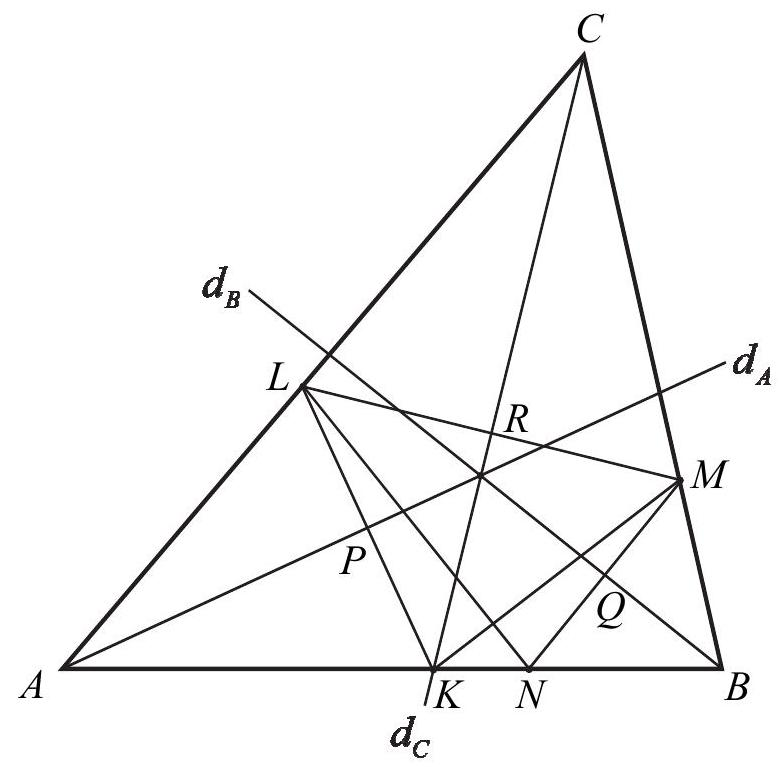
\includegraphics[max width=\textwidth, center]{2025_02_07_a13180f11f288af0ed0dg-05}

Wówczas $2 \alpha+2 \beta+2 \gamma=180^{\circ}$, stąd $\alpha+\beta+\gamma=90^{\circ}$. Wtedy

$$
|\Varangle K A P|=\alpha, \text { zatem }|\Varangle A K P|=90^{\circ}-\alpha \text { i }|\Varangle L K N|=180^{\circ}-\left(90^{\circ}-\alpha\right)=90^{\circ}+\alpha
$$

oraz

$$
\begin{aligned}
& |\Varangle C M R|=90^{\circ}-\gamma \text { oraz }|\Varangle B M Q|=90^{\circ}-\beta, \\
& \text { zatem }|\Varangle L M N|=180^{\circ}-\left(90^{\circ}-\gamma\right)-\left(90^{\circ}-\beta\right)=\beta+\gamma .
\end{aligned}
$$

Suma kątów $L K N$ i $L M N$ jest więc równa

$$
|\Varangle L K N|+|\Varangle L M N|=\left(90^{\circ}+\alpha\right)+(\beta+\gamma)=\alpha+\beta+\gamma+90^{\circ}=180^{\circ} .
$$

To oznacza, że na czworokącie $K N M L$ można opisać okrąg.

\section*{II sposób - symetralne}
\begin{center}
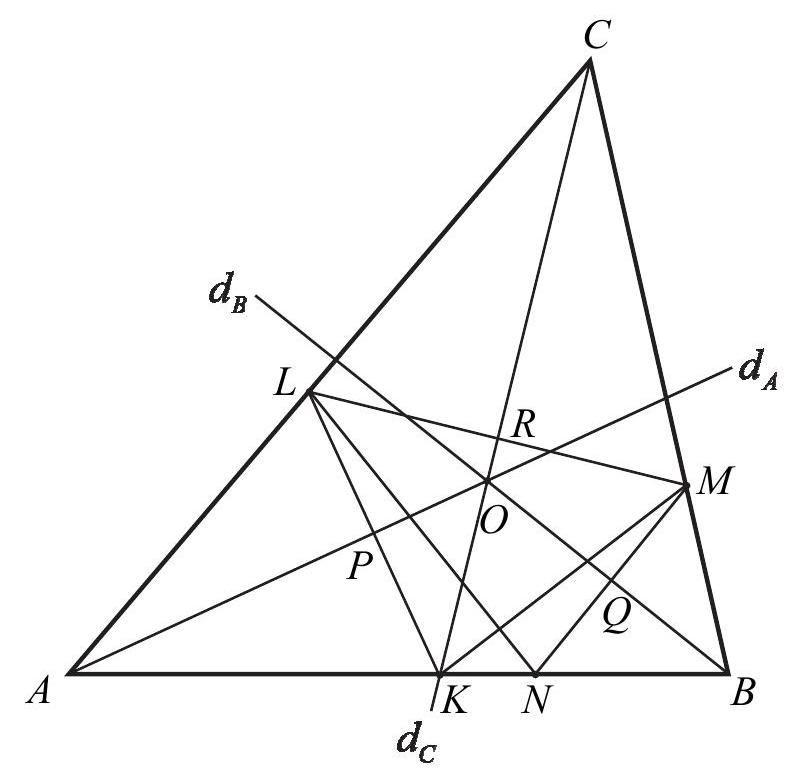
\includegraphics[max width=\textwidth]{2025_02_07_a13180f11f288af0ed0dg-06}
\end{center}

Rozważmy trójkąt $K L M$. Z definicji symetrii osiowej wynika, że dwusieczna $d_{A}$ jest symetralną boku $K L$. Analogicznie dwusieczna $d_{C}$ jest symetralną boku LM. Symetralne boków trójkąta przecinają się w jednym punkcie, który jest środkiem okręgu opisanego na tym trójkącie - oznaczmy go przez $O$. Czyli punkt wspólny dwusiecznych $d_{A}$ i $d_{C}$ (symetralnych boków trójkąta $K L M$ ) jest środkiem okręgu, którego promieniem jest w szczególności odcinek $O L$.\\
Podobnie rozważmy trójkąt $L M N$. Z definicji symetrii osiowej wynika, że dwusieczna $d_{C}$ jest symetralną boku $L M$. Analogicznie dwusieczna $d_{B}$ jest symetralną boku $M N$. Punkt wspólny tych dwusiecznych (symetralnych) jest tym samym punktem, o którym była mowa wyżej i jest oczywiście środkiem okręgu opisanego na trójkącie $L M N$. Zatem musi to być ten sam okrąg. Wszystkie wierzchołki czworokąta KNML leżą na tym okręgu. To kończy dowód.

\section*{III sposób - równość promieni}
Oznaczmy przez $O$ punkt przecięcia się dwusiecznych kątów trójkąta $A B C$, punkt wspólny dwusiecznej $d_{A}$ i odcinka $K L$ przez $P$, dwusiecznej $d_{C}$ i odcinka $L M$ przez $R$ oraz dwusiecznej $d_{B}$ i odcinka $M N$ przez $Q$.\\
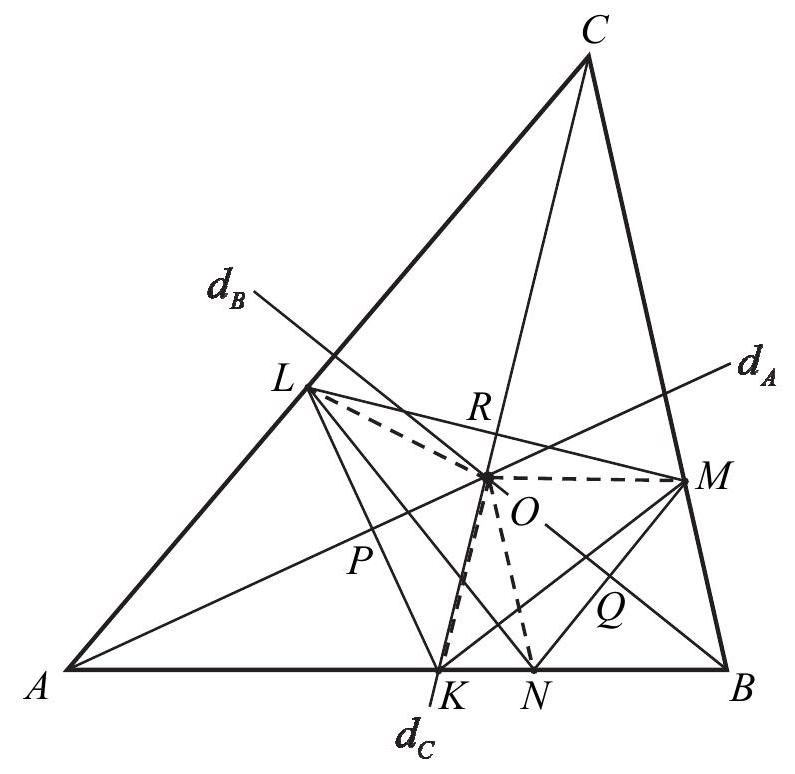
\includegraphics[max width=\textwidth, center]{2025_02_07_a13180f11f288af0ed0dg-07}

Z definicji symetrii osiowej i z treści zadania wynika, że $|K P|=|L P|$ oraz $K L \perp A O$. Oznacza to, że trójkąty $O P K$ i $O P L$ są prostokątne, mają wspólną przyprostokątną $O P$ oraz pozostałe przyprostokątne są równej długości. Są to więc trójkąty przystające (na mocy cechy bkb przystawania trójkątów). Stąd wynika, że $|O L|=|O K|$. Analogicznie trójkąty $O R L$ i $O R M$ są przystające oraz trójkąty $O Q M$ i $O Q N$ są przystające, a w konsekwencji $|O L|=|O M|$ oraz $|O M|=|O N|$. Zatem punkt $O$ jest więc równooddalony od wszystkich wierzchołków czworokąta $K N M L$, a to oznacza, że na tym czworokącie można opisać okrąg.

\section*{Schemat punktowania}
Rozwiązanie, w którym jest istotny postęp\\
1 p.\\
Zdający

\begin{itemize}
  \item wyznaczy miarę jednego z kątów czworokąta $K N M L$ w zależności od miar kątów trójkąta $A B C$, np.: $|\Varangle L K N|=90^{\circ}+\alpha$\\
albo
  \item zapisze, że prosta zawierająca dwusieczną kąta trójkąta $A B C$ jest symetralną jednego z odcinków $K L, L M, M N$\\
albo
  \item zapisze jedną lub dwie równości spośród: $|O L|=|O K|,|O L|=|O M|,|O M|=|O N|$ i na tym zakończy lub dalej popełnia błędy.
\end{itemize}

\section*{Pokonanie zasadniczych trudności zadania}
Zdający

\begin{itemize}
  \item wyznaczy miary dwóch przeciwległych kątów czworokąta $K N M L$ w zależności od miar kątów trójkąta $A B C$, np.: $|\Varangle L K N|=90^{\circ}+\alpha$ i $|\Varangle L M N|=\beta+\gamma$\\
albo
  \item zapisze, że punkt przecięcia dwusiecznych kątów trójkąta $A B C$ jest środkiem okręgu opisanego na trójkącie $K L M$ lub na trójkącie $L M N$, lub że jest punktem przecięcia symetralnych trzech boków czworokąta $K N M L$\\
albo
  \item zapisze i uzasadni jedną lub dwie równości spośród: $|O L|=|O K|,|O L|=|O M|$, $|O M|=|O N|$
\end{itemize}

\section*{Uwaga}
Jeżeli zdający zapisze wszystkie równości $|O L|=|O K|,|O L|=|O M|,|O M|=|O N|$ i stąd wyciągnie wniosek, że punkt $O$ jest środkiem okręgu opisanego na czworokącie $K N M L$, ale nie uzasadni żadnej z tych równości (lub uzasadnienie nie będzie pełne), to otrzymuje 2 punkty.

\section*{Rozwiązanie pełne}
Zdający przeprowadzi pełne rozumowanie.

\section*{Uwagi}
\begin{enumerate}
  \item Jeżeli zdający przeprowadza dowód $z$ wykorzystaniem bilansu kątów i korzysta z równości kątów w trójkątach równoramiennych, to może otrzymać 3 punkty także w przypadku, gdy bez stosownego komentarza korzysta z faktu, że trójkąty są równoramienne.
  \item Jeżeli zdający
\end{enumerate}

\begin{itemize}
  \item uzależni wszystkie kąty trójkąta $A B C$ oraz jeden z kątów czworokąta $K N M L$\\
albo
  \item uzależni jeden z kątów $L K N, K N M$ i jeden z kątów $K L M, N M L$\\
od kątów $\alpha=\Varangle A K L=\Varangle A L K, \beta=\Varangle B M L=\Varangle B L M$ i $\gamma=\Varangle C L M=\Varangle C M L$, to otrzymuje 1 punkt.
\end{itemize}

\begin{enumerate}
  \setcounter{enumi}{2}
  \item Jeżeli zdający
\end{enumerate}

\begin{itemize}
  \item wyznaczy 2 przeciwległe kąty czworokąta $K N M L$ w zależności od $\alpha, \beta, \gamma$ i wykaże, że $\alpha+\beta+\gamma=180^{\circ}$\\
albo
  \item wyznaczy wszystkie kąty czworokąta KNML i obliczy sumę dwóch przeciwległych kątów czworokąta $K N M L$,\\
to otrzymuje 2 punkty.
\end{itemize}

\section*{Zadanie 8. (0-3)}
\begin{center}
\begin{tabular}{|l|l|}
\hline
 & \begin{tabular}{l}
2. Wyrażenia algebraiczne. Zdajaccy rozkłada wielomian \\
na czynniki, stosując wzory skróconego mnożenia lub \\
\end{tabular} \\
V. Rozumowanie & wyłączajaç wspólny czynnik przed nawias (R2.3). \\
i argumentacja. & SP2. Działania na liczbach naturalnych. Zdajacy \\
 & rozpoznaje liczby naturalne podzielne przez 2,3 \\
(SP2.3). &  \\
\end{tabular}
\end{center}

\section*{Przykładowe rozwiązania}
\section*{I sposób}
Zauważmy, że $k^{3} m-k m^{3}=k m\left(k^{2}-m^{2}\right)=k m(k+m)(k-m)$.\\
Rozwiązanie zadania składa się z dwóch etapów:

\begin{itemize}
  \item uzasadnienie podzielności przez 2;
  \item uzasadnienie podzielności przez 3.
\end{itemize}

Podzielność przez 2.\\
Gdy którakolwiek z liczb $k, m$ jest parzysta, to iloczyn $k m\left(k^{2}-m^{2}\right)$ jest parzysty, a gdy obie liczby $k, m$ są nieparzyste, to ich suma $k+m$ jest liczbą parzystą, więc iloczyn\\
$k m(k+m)(k-m)$ jest podzielny przez 2 .\\
Podzielność przez 3. (I sposób)\\
Dowód przeprowadzimy w czterech rozłącznych sytuacjach: A, B, C, D.\\
A. Którakolwiek z liczb $k, m$ jest podzielna przez 3

Wtedy iloczyn $k m\left(k^{2}-m^{2}\right)$ jest podzielny przez 3 .\\
B. Obie liczby $k, m$ przy dzieleniu przez 3 dają resztę 1

Wtedy liczba $k-m$ jest podzielna przez 3, więc iloczyn $k m(k+m)(k-m)$ jest podzielny przez 3 .\\
C. Obie liczby $k, m$ przy dzieleniu przez 3 dają resztę 2

Wtedy liczba $k-m$ jest podzielna przez 3, więc iloczyn $k m(k+m)(k-m)$ jest podzielny przez 3 .\\
D. Jedna $z$ liczb $k, m$ przy dzieleniu przez 3 daje resztę 1 , a druga przy dzieleniu przez 3 daje resztę 2\\
Wtedy liczba $k+m$ jest podzielna przez 3, więc iloczyn $k m(k+m)(k-m)$ jest podzielny przez 3 .

\section*{Podzielność przez 3. (II sposób)}
Dowód przeprowadzimy w dwóch rozłącznych sytuacjach: E, F.\\
E. Którakolwiek z liczb $k, m$ jest podzielna przez 3.

Wtedy iloczyn $k m\left(k^{2}-m^{2}\right)$ jest podzielny przez 3 .\\
F. Żadna z liczb $k, m$ nie jest podzielna przez 3 .

Wtedy kwadrat każdej z nich przy dzieleniu przez 3 daje resztę 1, więc różnica $k^{2}-m^{2}$ jest podzielna przez 3.

Wykazaliśmy zatem, że liczba $k^{3} m-k m^{3}$ jest podzielna przez 2 i przez 3, więc jest podzielna przez $2 \cdot 3$, czyli przez 6. To kończy dowód.

\section*{II sposób}
Zauważmy, że\\
$k^{3} m-k m^{3}=k m\left(k^{2}-1+1-m^{2}\right)=k m\left(k^{2}-1\right)-k m\left(m^{2}-1\right)=k m(k-1)(k+1)-k m(m-1)(m+1)$\\
Iloczyn $k(k-1)(k+1)$ to iloczyn trzech kolejnych liczb całkowitych, więc dokładnie jedna z nich jest podzielna przez 3 i co najmniej jedna jest podzielna przez 2, więc iloczyn jest podzielny przez 2 i przez 3, a więc jest podzielny przez 6. Analogicznie iloczyn $m(m-1)(m+1)$ jest podzielny przez 6. Różnica dwóch liczb podzielnych przez 6 jest podzielna przez 6. To kończy dowód.\\
Schemat punktowania\\
Zdający otrzymuje\\
jeśli

\begin{itemize}
  \item uzasadni podzielność przez 2\\
albo
  \item uzasadni podzielność przez 3 w dwóch przypadkach spośród $\mathrm{A}, \mathrm{B}, \mathrm{C}, \mathrm{D}$,\\
albo
  \item uzasadni podzielność przez 3 w przypadku F.
\end{itemize}

Zdający otrzymuje 2 p.\\
jeśli

\begin{itemize}
  \item uzasadni podzielność przez 2 i uzasadni podzielność przez 3 w dwóch przypadkach spośród A, B, C, D\\
albo
  \item uzasadni podzielność przez 2 i uzasadni podzielność przez 3 w przypadku F ,\\
albo
  \item uzasadni podzielność przez 3,\\
albo
  \item zapisze liczbe $k^{3} m-k m^{3}$ w postaci $k m(k-1)(k+1)-k m(m-1)(m+1)$.
\end{itemize}

Zdający otrzymuje 3 p.\\
przeprowadzi pełne rozumowanie uzasadniające podzielność przez 6 .

\section*{Uwagi}
\begin{enumerate}
  \item Akceptujemy sytuacje, w której zdający stwierdza bez uzasadnienia, że iloczyn trzech kolejnych liczb całkowitych jest podzielny przez 6 oraz różnica liczb podzielnych przez 6 jest podzielna przez 6.
  \item Jeżeli zdający rozważa reszty z dzielenia liczb $k$ i $m$ przez 6 i udowodni podzielność przez 6 w jednym z poniższych 5 przypadków:
\end{enumerate}

\begin{itemize}
  \item dokładnie jedna z liczb $k, m$ jest podzielna przez 6 lub obie liczby $k, m$ dają przy dzieleniu przez 6 tę samą resztę;
  \item żadna z liczb $k, m$ nie jest podzielna przez 6 , a o podzielności liczby $k^{3} m-k m^{3}$ można wnioskować na podstawie iloczynu liczb $k, m$;
  \item żadna z liczb $k, m$ nie jest podzielna przez 6 , a o podzielności liczby $k^{3} m-k m^{3}$ można wnioskować na podstawie sumy liczb $k, m$;
  \item żadna z liczb $k, m$ nie jest podzielna przez 6 , a o podzielności liczby $k^{3} m-k m^{3}$ można wnioskować na podstawie sumy i iloczynu liczb $k, m$;
  \item żadna z liczb $k, m$ nie jest podzielna przez 6 , a o podzielności liczby $k^{3} m-k m^{3}$ można wnioskować na podstawie różnicy i iloczynu liczb $k, m$, to otrzymuje 1 punkt.
\end{itemize}

\begin{enumerate}
  \setcounter{enumi}{2}
  \item Jeżeli zdający rozważa reszty z dzielenia liczb $k$ i $m$ przez 6 i udowodni podzielność przez 6 w trzech z poniższych 5 przypadków:
\end{enumerate}

\begin{itemize}
  \item dokładnie jedna z liczb $k, m$ jest podzielna przez 6 lub obie liczby $k, m$ dają przy dzieleniu przez 6 tę samą resztę;
  \item żadna z liczb $k, m$ nie jest podzielna przez 6 , a o podzielności liczby $k^{3} m-k m^{3}$ można wnioskować na podstawie iloczynu liczb $k, m$;
  \item żadna z liczb $k, m$ nie jest podzielna przez 6 , a o podzielności liczby $k^{3} m-k m^{3}$ można wnioskować na podstawie sumy liczb $k, m$;
  \item żadna z liczb $k, m$ nie jest podzielna przez 6 , a o podzielności liczby $k^{3} m-k m^{3}$ można wnioskować na podstawie sumy i iloczynu liczb $k, m$;
  \item żadna z liczb $k, m$ nie jest podzielna przez 6 , a o podzielności liczby $k^{3} m-k m^{3}$ można wnioskować na podstawie różnicy i iloczynu liczb $k, m$, to otrzymuje 2 punkty.
\end{itemize}

Zadanie 9. (0-4)

\begin{center}
\begin{tabular}{|l|l|}
\hline
 & \begin{tabular}{l}
10. Elementy statystyki opisowej. Teoria \\
prawdopodobieństwa i kombinatoryka. Zdający \\
wykorzystuje wzory na liczbę permutacji, kombinacji, \\
III. Modelowanie \\
matematyczne. \\
\end{tabular} \\
\begin{tabular}{l}
wariacji i wariacji z powtórzeniami do zliczania \\
obiektów w bardziej złożonych sytuacjach \\
kombinatorycznych (R10.1). Zdający oblicza \\
prawdopodobieństwa w prostych sytuacjach, stosując \\
klasyczną definicję prawdopodobieństwa (10.3). \\
\end{tabular} &  \\
\hline
\end{tabular}
\end{center}

\section*{Przykładowe rozwiązania}
\section*{I sposób}
Zdarzeniami elementarnymi są permutacje (bez powtórzeń) zbioru ośmioelementowego $\{1,2,3,4,5,6,7,9\}$.\\
Liczba wszystkich zdarzeń elementarnych jest równa $|\Omega|=8$ !.\\
Niech $A$ będzie zdarzeniem, polegającym na tym, że żadne dwie liczby parzyste nie są sąsiednimi wyrazami utworzonego ciągu. Ustalmy liczbę wszystkich zdarzeń elementarnych sprzyjających zdarzeniu $A$.

\section*{I metoda}
W zbiorze $Z$ jest 5 liczb nieparzystych, więc możemy je ustawić w ciąg na 5! sposobów. Otrzymamy wtedy sytuację:\\
(1) n (2) n (3) n (4) n (5) n (6)

Pierwszą z pozostałych liczb (parzystych) zbioru $Z$ możemy ustawić na jednym z sześciu miejsc (1)\_ - (6)\_, drugą na jednym z pozostałych pięciu, a trzecią na jednym z pozostałych czterech.\\
Zatem $|A|=5!\cdot 6 \cdot 5 \cdot 4$.

\section*{II metoda}
W zbiorze $Z$ jest 5 liczb nieparzystych, więc możemy je ustawić w ciąg na 5! sposobów.\\
Otrzymamy wtedy sytuację:\\
(1) n (2) n (3) n (4) n (5) n (6)

Trzy pozostałe liczby (parzyste) ze zbioru $Z$ musimy ustawić na wybranych trzech miejscach spośród sześciu miejsc \textit{(1)} - (6). Te trzy miejsca możemy wybrać na $\binom{6}{3}$ sposobów. Na tych trzech ustalonych miejscach możemy trzy liczby parzyste ze zbioru $Z$ ustawić na 3! sposobów.\\
Zatem $|A|=5!\cdot\binom{6}{3} \cdot 3$ !.\\
III metoda (ustalenie kolejności parzystych, a następnie ustalenie pozycji parzystych)\\
W zbiorze $Z$ mamy 3 liczby parzyste: 2 , 4 , 6 . Możemy ustawić je w kolejności na $3!=6$ sposobów. Jedną z takich możliwości jest kolejność: 2, 4, 6 .\\
Wypiszmy wszystkie przypadki ustawienia tych trzech liczb w kolejności 2, 4, 6 w ciągu\\
8-wyrazowym:\\
(a) 2 na pierwszym miejscu

$$
\begin{aligned}
& 2-4-6---, 2-4--6--, 2-4---6-, 2-4----6,2--4-6--, \\
& 2--4--6-, 2-4---6,2--4-6-, 2--4--6,2---4-6,
\end{aligned}
$$

(b) 2 na drugim miejscu\\
$-2-4-6--,-2-4--6-,-2-4---6,-2--4-6-,-2--4--6$, $-2---4-6$,\\
(c) 2 na trzecim miejscu

$$
--2-4-6-,--2-4--6,--2--4-6,
$$

(d) 2 na czwartym miejscu

$$
---2-4-6 .
$$

Łącznie mamy 20 przypadków ustawienia w ciągu 8-wyrazowym trzech liczb parzystych $-2,4,6-$ w kolejności $2,4,6$.\\
Ponieważ mamy 6 możliwości ustalenia kolejności dla trzech liczb 2, 4, 6, więc liczby parzyste ze zbioru $Z$ możemy ustawić na $6 \cdot 20$ sposobów.\\
Do ustawionych liczb parzystych na wolne miejsca ustawiamy liczby nieparzyste, a możemy to zrobić na 5! sposobów.\\
Zatem $|A|=6 \cdot 20 \cdot 5!$.\\
IV metoda (ustalenie pozycji parzystych)\\
Wypiszmy wszystkie przypadki wyboru trzech miejsc, spośród ośmiu, dla liczb parzystych, z uwzględnieniem warunku, że żadne dwie parzyste nie sąsiadują ze sobą.\\
(a) pierwsza liczba parzysta na pierwszym miejscu

$$
\begin{aligned}
& \mathrm{p}-\mathrm{p}-\mathrm{p}---, \mathrm{p}-\mathrm{p}-\mathrm{p}--\mathrm{p}-\mathrm{p}---\mathrm{p}-, \mathrm{p}-\mathrm{p}---\mathrm{p}, \mathrm{p}--\mathrm{p}-\mathrm{p}-- \\
& \mathrm{p}--\mathrm{p}--\mathrm{p}-, \mathrm{p}-\mathrm{p}--\mathrm{p}, \mathrm{p}--\mathrm{p}-\mathrm{p}-, \mathrm{p}--\mathrm{p}--\mathrm{p}, \mathrm{p}---\mathrm{p}-\mathrm{p},
\end{aligned}
$$

(b) pierwsza liczba parzysta na drugim miejscu

$$
\begin{aligned}
& -\mathrm{p}-\mathrm{p}-\mathrm{p}--,-\mathrm{p}-\mathrm{p}--\mathrm{p}-,-\mathrm{p}-\mathrm{p}---\mathrm{p},-\mathrm{p}--\mathrm{p}-\mathrm{p}-,-\mathrm{p}--\mathrm{p}--\mathrm{p} \\
& -\mathrm{p}--\mathrm{p}-\mathrm{p}
\end{aligned}
$$

(c) pierwsza liczba parzysta na trzecim miejscu

$$
--\mathrm{p}-\mathrm{p}-\mathrm{p}-,--\mathrm{p}-\mathrm{p}--\mathrm{p},--\mathrm{p}--\mathrm{p}-\mathrm{p},
$$

(d) pierwsza liczba parzysta na czwartym miejscu

$$
---\mathrm{p}-\mathrm{p}-\mathrm{p} .
$$

Łącznie mamy 20 przypadków ustalenia w ciągu 8-wyrazowym pozycji liczb parzystych.\\
Zatem $|A|=20 \cdot 3!5$ !.

Uwaga! Te same przypadki wyboru uzyskamy, wypisując wszystkie ustawienia liczb parzystych i nieparzystych przy założeniu, że rozpoczynamy najpierw od liczby parzystej (10 przypadków), a następnie od nieparzystej (kolejne 10 przypadków). Ponadto należy pamiętać, że przedstawione tu przypadki ustawień liczb parzystych (a tym samym i nieparzystych) mogą być przedstawione jako gałęzie drzewa probabilistycznego z 20 gałęziami.

\section*{$V$ metoda (przerwy między parzystymi)}
Trzy liczby parzyste musimy rozdzielić pięcioma nieparzystymi, przy czym nieparzyste możemy umieszczać także przed wszystkimi parzystymi lub po wszystkich parzystych. Mamy zatem 4 usytuowania dla liczb nieparzystych.\\
Wypiszmy najpierw przypadki uwzględniające liczbę pozycji dla liczb nieparzystych w poszczególnych usytuowaniach (cyfra oznacza liczbę miejsc zajętych przez liczby nieparzyste, litera $p$ oznacza liczbę parzystą).\\
$0-p-1-p-1-p-3,0-p-1-p-2-p-2,0-p-1-p-3-p-1,0-p-1-p-4-p-0,0-p-2-p-1-p-2,0-p-2-p-2-p-1$,\\
$0-\mathrm{p}-2-\mathrm{p}-3-\mathrm{p}-0, \quad 0-\mathrm{p}-3-\mathrm{p}-1-\mathrm{p}-1, \quad 0-\mathrm{p}-3-\mathrm{p}-2-\mathrm{p}-0, \quad 0-\mathrm{p}-4-\mathrm{p}-1-\mathrm{p}-0, \quad 1-\mathrm{p}-1-\mathrm{p}-1-\mathrm{p}-1,1-\mathrm{p}-1-\mathrm{p}-2-\mathrm{p}-1$, 1-p-1-p-3-p-0, 1-p-2-p-1-p-1, 1-p-2-p-2-p-0, 1-p-3-p-1-p-0, 2-p-1-p-1-p-1, 2-p-1-p-2-p-0, 2-p-2-p-1-p-0, 3-p-1-p-1-p-0\\
Łącznie mamy 20 takich przypadków.\\
Zatem $|A|=20 \cdot 3!5$ !.\\
Obliczamy prawdopodobieństwo:

$$
P(A)=\frac{20 \cdot 3!\cdot 5!}{8!}=\frac{10}{28}=\frac{5}{14} .
$$

\section*{II sposób (zdarzenie przeciwne)}
Zdarzeniami elementarnymi są permutacje (bez powtórzeń) zbioru ośmioelementowego $\{1,2,3,4,5,6,7,9\}$.\\
Liczba wszystkich zdarzeń elementarnych jest równa $|\Omega|=8$ !\\
Niech $A$ będzie zdarzeniem, polegającym na tym, że żadne dwie liczby parzyste nie są sąsiednimi wyrazami utworzonego ciągu.\\
Zdarzeniem przeciwnym $A^{\prime}$ jest otrzymanie w wyniku permutacji zbioru $Z$ ciągu, w którym liczby parzyste są sąsiednimi wyrazami ciągu, tzn.\\
I: wszystkie trzy liczby parzyste będą kolejnymi wyrazami ciągu\\
albo\\
II. dwie liczby parzyste będą kolejnymi wyrazami ciągu, a trzecia liczba parzysta nie będzie sąsiadować z żadną z nich.\\
W sytuacji I miejsca dla liczb parzystych wybieramy na 6 sposobów, ustawiamy na tych miejscach liczby parzyste na 3! sposobów, a pozostałe liczby ustawiamy na pięciu miejscach na 5! sposobów.\\
W sytuacji II. dla sąsiadujących liczb parzystych wybieramy miejsca na 7 sposobów:\\
$\mathrm{m}_{1}$ i $\mathrm{m}_{2}, \mathrm{~m}_{2}$ i $\mathrm{m}_{3}, \mathrm{~m}_{3}$ i $\mathrm{m}_{4}, \mathrm{~m}_{4}$ i $\mathrm{m}_{5}, \mathrm{~m}_{5} \mathrm{i} \mathrm{m}_{6}, \mathrm{~m}_{6}$ i $\mathrm{m}_{7}, \mathrm{~m}_{7}$ i $\mathrm{m}_{8}$.\\
Miejsce dla trzeciej parzystej liczby możemy wybrać: na 5 sposobów wtedy, gdy parzyste liczby sąsiadują na miejscach $\mathrm{m}_{1}$ i $\mathrm{m}_{2}$ albo na miejscach $\mathrm{m}_{7}$ i m8 oraz na 4 sposoby w każdej z pozostałych możliwości.\\
Liczby parzyste możemy rozstawić na wybranych miejscach na 3! sposobów, a pozostałe liczby ustawiamy na pięciu miejscach na 5 ! sposobów.\\
Wszystkich zdarzeń elementarnych sprzyjających zdarzeniu $A^{\prime}$ jest:\\
$6 \cdot 3!\cdot 5!+2 \cdot 5 \cdot 3!\cdot 5!+5 \cdot 4 \cdot 3!\cdot 5$ !.

Obliczamy prawdopodobieństwo zdarzenia $A$ :\\
$P(A)=1-P\left(A^{\prime}\right)=1-\frac{36 \cdot 3!\cdot 5!}{8!}=1-\frac{36 \cdot 6}{6 \cdot 7 \cdot 8}=1-\frac{36}{56}=\frac{20}{56}=\frac{5}{14}$.\\
Uwaga! Zdający może wypisywać przypadki, w których wystąpią zdarzenia elementarne sprzyjające zdarzeniu $A^{\prime}$, stosując metody analogiczne do metod III, IV, V z I sposobu rozwiązania, i uwzględnić 36 rozłącznych przypadków.

\section*{Schemat punktowania}
\section*{Rozwiązanie, w którym postęp jest niewielki, ale konieczny na drodze do pełnego rozwiązania \\
 1 p. \\
 Zdający}
\begin{itemize}
  \item zapisze $|\Omega|=8$ !\\
albo
  \item wypisze przynajmniej 11 różnych przypadków spośród 20, gdy rozpatruje zdarzenie $A$ albo
  \item wypisze przynajmniej 19 różnych przypadków spośród 36, gdy rozpatruje zdarzenie $A^{\prime}$, albo
  \item zapisze, że jest $\binom{6}{3}$ lub $6 \cdot 5 \cdot 4$ przypadków, gdy rozpatruje zdarzenie $A$ (lub $6+2 \cdot 5+5 \cdot 4$ przypadków, gdy rozpatruje zdarzenie $A^{\prime}$ ),\\
albo
  \item zapisze iloczyn $3!5$ ! lub w inny sposób zaznaczy uwzględnienie iloczynu $3!\cdot 5$ !, wynikającego z permutacji liczb parzystych i liczb nieparzystych na wybranych dla nich miejscach,\\
albo
  \item narysuje drzewo z wyróżnionymi co najmniej 11 różnymi istotnymi gałęziami odpowiadającymi zdarzeniu $A$ (albo z wyróżnionymi co najmniej 19 różnymi istotnymi gałęziami odpowiadającymi zdarzeniu $A^{\prime}$ ),\\
albo
  \item narysuje niepełne drzewo (może wystąpić brak istotnych gałęzi odpowiadających zdarzeniu $A$ lub $A^{\prime}$ ), ale na wszystkich odcinkach co najmniej jednej gałęzi zapisze prawdopodobieństwa, przy czym gałąź ta musi uwzględniać jeden z przypadków: wylosowano 3 parzyste liczby lub wylosowano 7 liczb\\
i na tym zakończy lub dalej popełnia błędy.\\
Rozwiązanie, w którym jest istotny postęp\\
Zdający
  \item zapisze $|\Omega|=8$ ! i wypisze przynajmniej 11 różnych przypadków spośród 20, gdy rozpatruje zdarzenie $A$,\\
albo
  \item zapisze $|\Omega|=8$ ! i wypisze przynajmniej 19 różnych przypadków spośród 36, gdy rozpatruje zdarzenie $A^{\prime}$,\\
albo
  \item zapisze $|\Omega|=8$ ! i zapisze, że jest $\binom{6}{3}$ lub $6 \cdot 5 \cdot 4$ przypadków, gdy rozpatruje zdarzenie $A$ (lub $6+2 \cdot 5+5 \cdot 4$ przypadków, gdy rozpatruje zdarzenie $A^{\prime}$ ),\\
albo
  \item zapisze $|A|=\binom{6}{3} \cdot 3!\cdot 5!$ lub $|A|=6 \cdot 5 \cdot 4 \cdot 5$ ! lub $|A|=20 \cdot 3!\cdot 5$ ! lub
\end{itemize}

$$
\left|A^{\prime}\right|=(6+2 \cdot 5+5 \cdot 4) \cdot 3!\cdot 5!\operatorname{lub}\left|A^{\prime}\right|=36 \cdot 3!\cdot 5!
$$

albo

\begin{itemize}
  \item narysuje drzewo $z$ wyróżnionymi co najmniej 11 różnymi istotnymi gałęziami odpowiadającymi zdarzeniu $A$ (albo z wyróżnionymi co najmniej 19 różnymi istotnymi gałęziami odpowiadającymi zdarzeniu $A^{\prime}$ ) i na wszystkich odcinkach co najmniej jednej gałęzi zapisze prawdopodobieństwa, przy czym gałąź ta musi uwzględniać jeden z przypadków: wylosowano 3 parzyste liczby lub wylosowano 7 liczb i na tym zakończy lub dalej popełnia błędy.\\
Pokonanie zasadniczych trudności zadania\\
Zdający
  \item zapisze $|\Omega|=8$ ! i zapisze $|A|=\binom{6}{3} \cdot 3!\cdot 5$ ! lub $|A|=6 \cdot 5 \cdot 4 \cdot 5$ ! lub $|A|=20 \cdot 3!\cdot 5$ !
\end{itemize}

$$
\text { lub }\left|A^{\prime}\right|=(6+2 \cdot 5+5 \cdot 4) \cdot 3!\cdot 5!\text { lub }\left|A^{\prime}\right|=36 \cdot 3!\cdot 5!
$$

albo

\begin{itemize}
  \item zapisze prawdopodobieństwo zdarzenia $A$ (albo $A^{\prime}$ ) zgodnie z „metodą drzewkową".
\end{itemize}

Rozwiązanie pełne\\
Zdający obliczy prawdopodobieństwo: $P(A)=\frac{5}{14}$.

\section*{Uwagi}
\begin{enumerate}
  \item Możemy też rozpatrywać model probabilistyczny, w którym zdarzeniem elementarnym jest 3 elementowy podzbiór zbioru 8 elementowego (nie uwzględniamy wówczas kolejności ustawienia liczb nieparzystych ani kolejności ustawienia liczb parzystych, a jedynie pozycje zajmowane przez te liczby). Wtedy $|\Omega|=\binom{8}{3}=56,|A|=\binom{6}{3}=20$, $P(A)=\frac{5}{14}$.
  \item Jeżeli zdający błędnie założy, że podany w treści zadania ośmioelementowy zbiór $Z$ zawiera 4 liczby parzyste i 4 liczby nieparzyste (np. założy, że zbiór $Z$ zawiera liczbę 8 zamiast 9) i rozwiąże zadanie do końca, otrzymując $P(A)=\frac{5 \cdot 4!\cdot 4!}{8!}=\frac{1}{14}$, to otrzymuje 2 punkty. Zdający otrzymuje w tej sytuacji 1 punkt tylko za zapisanie $|\Omega|=8$ !.
  \item Jeżeli zdający błędnie założy, że podany w treści zadania zbiór $Z$ jest 9-elementowy (i zawiera 4 liczby parzyste i 5 liczby nieparzystych) i konsekwentnie rozwiąże zadanie do końca, to otrzymuje 3 punkty.
  \item Jeżeli zdający zapisze $|\Omega|=8$ ! oraz rozpatrując zdarzenie $A^{\prime}$ rozważy trzy sytuacje:\\
I. wszystkie trzy liczby parzyste są kolejnymi wyrazami ciągu;\\
II. dwie liczby parzyste są dwoma skrajnymi (pierwszym i drugim lub siódmym i ósmym) wyrazami ciągu, a trzecia liczba parzysta nie sąsiaduje bezpośrednio z żadną z nich;\\
III. dwie liczby parzyste są dwoma kolejnymi, ale nie skrajnymi wyrazami ciągu, a trzecia parzysta nie sąsiaduje bezpośrednio z żadną z nich\\
oraz zapisze sposób zliczania tych ciągów w każdej z tych trzech sytuacji, uwzględniający permutacje liczb parzystych i liczb nieparzystych i jednoczenie gwarantujący to, że żaden ciąg nie zostanie policzony wielokrotnie;\\
a ponadto nie ustali poprawnej liczby wszystkich zdarzeń elementarnych sprzyjających zdarzeniu $A^{\prime}$, to otrzymuje 2 punkty.
  \item Jeżeli zdający rozważa zdarzenie $A$ i wypisuje przynajmniej 12 przypadków, ale jeden z nich zapisuje dwukrotnie, to otrzymuje przynajmniej 1 punkt. Dotyczy to także sytuacji wypisania 21 przypadków.
\end{enumerate}

Zadanie 10. (0-4)

\begin{center}
\begin{tabular}{|l|l|}
\hline
\multirow{4}{*}{IV. Użycie i tworzenie strategii.} & \begin{tabular}{l}
9. Stereometria. Zdający rozpoznaje w walcach \\
i w stożkach kạt między odcinkami oraz kąt między \\
odcinkami i płaszczyznami (9.3). \\
3. Równania i nierówności. Zdający rozwiązuje \\
równania kwadratowe z jedną niewiadomą (3.4). \\
\end{tabular} \\
\hline
\end{tabular}
\end{center}

\section*{Przykładowe rozwiązanie}
Przekrojem osiowym stożka jest trapez równoramienny $A B C D$. Niech $D E$ oznacza wysokość stożka opuszczoną z punktu $D$.\\
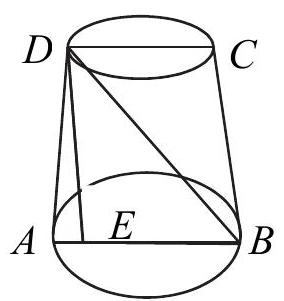
\includegraphics[max width=\textwidth, center]{2025_02_07_a13180f11f288af0ed0dg-16}

Po podstawieniu danych do wzoru na objętość otrzymujemy równanie kwadratowe

$$
\frac{1}{3} \pi \cdot 10 \cdot\left(6^{2}+6 R+R^{2}\right)=840 \pi .
$$

Stąd

$$
R^{2}+6 R-216=0 .
$$

Rozwiązując je, otrzymujemy

$$
\begin{gathered}
\Delta=36+4 \cdot 216=900, \sqrt{\Delta}=30 \\
R=\frac{-6-30}{2}=-18<0 \text { lub } R=\frac{-6+30}{2}=12 .
\end{gathered}
$$

Przekrojem osiowym tego stożka jest trapez równoramienny o podstawach długości 24 i 12 oraz wysokości 10. Długość odcinka $E B$ jest równa

$$
|E B|=R+r=12+6=18
$$

Z twierdzenia Pitagorasa dla trójkąta $B D E$ otrzymujemy

$$
|B D|=\sqrt{10^{2}+18^{2}}=\sqrt{424}=2 \sqrt{106} .
$$

Zatem $\cos |\Varangle D B E|=\frac{18}{2 \sqrt{106}}=\frac{9}{\sqrt{106}}$.

\section*{Schemat punktowania}
Rozwiązanie, w którym postęp jest niewielki, ale konieczny na drodze do pełnego rozwiązania 1 p.\\
Zdający wyznaczy promień $R$ większej podstawy: $R=12$ i na tym zakończy lub dalej popełni błędy.\\
Rozwiązanie, w którym jest istotny postęp ..... 2 p.

Zdający wyznaczy promień $R$ większej podstawy: $R=12$ i długość odcinka $E B:|E B|=18$, i na tym zakończy lub dalej popełni błędy.

\section*{Pokonanie zasadniczych trudności zadania}
\section*{Zdający obliczy}
\begin{itemize}
  \item długość przekątnej trapezu $|B D|=2 \sqrt{106}$\\
albo
  \item obliczy tangens kąta $D B E: \operatorname{tg}|\Varangle D B E|=\frac{5}{9}$\\
i na tym zakończy lub dalej popełni błędy.\\
Rozwiązanie petne 4 p.\\
Zdający obliczy $\cos |\Varangle D B E|=\frac{9}{\sqrt{106}}$.
\end{itemize}

\section*{Uwagi}
\begin{enumerate}
  \item Jeżeli zdający zapisze cosinus kąta nachylenia przekątnej przekroju osiowego tego stożka ściętego do jednej z jego podstaw w zależności od $R, r, H$ i na tym zakończy lub dalej popełnia błędy, to otrzymuje 2 punkty.
  \item Jeżeli zdający popełni błąd merytoryczny przy zastosowaniu twierdzenia Pitagorasa, pisząc np.: $|E B|^{2}+|B D|^{2}=|E D|^{2}$, albo popełni błąd merytoryczny przez zastosowanie nieistniejącego wzoru "pierwiastek sumy = suma pierwiastków", to może otrzymać co najwyżej 2 punkty za całe rozwiązanie.
  \item Jeżeli zdający błędnie przyjmie, że wysokością stożka jest odcinek $A D$, to może otrzymać co najwyżej 1 punkt, o ile poprawnie obliczy $R$.
  \item Jeżeli zdający realizuje strategię rozwiązania zadania i popełnia jedynie błędy rachunkowe, to może otrzymać $\mathbf{3}$ punkty, o ile popełnione błędy nie ułatwiają rozwiązania na żadnym etapie.
  \item Jeżeli zdający obliczy długość $R$ oraz długość ramienia trapezu, to może otrzymać 2 punkty. Jeżeli zdający obliczy długość $R$ oraz długość ramienia trapezu, a ponadto obliczy długośćc $B D$ i zapisze twierdzenie cosinusów, to może otrzymać 3 punkty.
  \item Jeżeli zdający błędnie przyjmuje, że średnica górnej podstawy stożka ściętego ma długość 6 , to otrzymuje co najwyżej $\mathbf{3}$ punkty.
  \item Jeżeli zdający błędnie przyjmuje, że długość rzutu prostokątnego ramienia trapezu na dłuższą podstawę to różnica średnic dolnej i górnej podstawy zamiast połowy tej różnicy i nie jest to błąd wynikający z rachunków, to otrzymuje co najwyżej 2 punkty za całe rozwiązanie.
\end{enumerate}

Zadanie 11. (0-4)

\begin{center}
\begin{tabular}{|l|l|}
\hline
IV. Użycie i tworzenie strategii. & \begin{tabular}{l}
6. Trygonometria. Zdający stosuje wzory na sinus \\
i cosinus sumy i różnicy kątów, sumę i różnicę sinusów \\
i cosinusów kątów (R6.5). Zdający rozwiązuje \\
równania i nierówności trygonometrycze (R6.6). \\
\end{tabular} \\
\hline
\end{tabular}
\end{center}

\section*{Przykładowe rozwiązanie}
Przekształcamy równanie w sposób równoważny

$$
\begin{gathered}
\sin 6 x+\cos 3 x=2 \sin 3 x+1, \\
2 \sin 3 x \cos 3 x+\cos 3 x=2 \sin 3 x+1, \\
\cos 3 x(2 \sin 3 x+1)=2 \sin 3 x+1, \\
(2 \sin 3 x+1)(\cos 3 x-1)=0, \\
\sin 3 x=-\frac{1}{2} \text { lub } \cos 3 x=1,
\end{gathered}
$$

Stąd $3 x=\frac{7 \pi}{6}+2 k \pi$ lub $3 x=\frac{11 \pi}{6}+2 k \pi$ lub $3 x=2 k \pi, k-$ liczba całkowita.\\
Zatem $x=\frac{7 \pi}{18}+\frac{2 k \pi}{3}$ lub $x=\frac{11 \pi}{18}+\frac{2 k \pi}{3}$ lub $x=\frac{2 k \pi}{3}$.\\
W przedziale $\langle 0, \pi\rangle$ mamy następujące rozwiązania równania: $x=\frac{7 \pi}{18}, x=\frac{11 \pi}{18}, x=0, x=\frac{2 \pi}{3}$.

\section*{Schemat punktowania}
\section*{Rozwiązanie, w którym postęp jest niewielki, ale konieczny na drodze do pełnego rozwiązania}
Zdający zastosuje wzór na sinus kąta podwojonego i zapisze równanie w postaci $2 \sin 3 x \cos 3 x+\cos 3 x=2 \sin 3 x+1$, i na tym zakończy lub dalej popełnia błędy.

Rozwiązanie, w którym jest istotny postęp\\
Zdający zapisze dwa równania $\sin 3 x=-\frac{1}{2}, \cos 3 x=1$.\\
Pokonanie zasadniczych trudności zadania 3 p.

\section*{Zdający}
\begin{itemize}
  \item zapisze wszystkie rozwiązania równań $\sin 3 x=-\frac{1}{2}$ oraz $\cos 3 x=1$ w zbiorze liczb rzeczywistych $x=\frac{7 \pi}{18}+\frac{2 k \pi}{3}$ lub $x=\frac{11 \pi}{18}+\frac{2 k \pi}{3}$ lub $x=\frac{2 k \pi}{3}$\\
albo
  \item zapisze dwa równania $\sin 3 x=-\frac{1}{2}$ oraz $\cos 3 x=1$ i jedno z nich rozwiąże w przedziale $\langle 0, \pi\rangle$\\
i na tym zakończy lub dalej popełnia błędy.
\end{itemize}

\section*{Rozwiązanie pehne}
Zdający zapisze wszystkie rozwiązania równania w przedziale $\langle 0, \pi\rangle: x=\frac{7 \pi}{18}, x=\frac{11 \pi}{18}$, $x=0, x=\frac{2 \pi}{3}$.

\section*{Uwagi}
\begin{enumerate}
  \item Jeżeli zdający poprawnie stosuje wzór na sinus kąta podwojonego, zapisze tylko jedno z równań $\cos 3 x=1, \sin 3 x=-\frac{1}{2}$, to otrzymuje
\end{enumerate}

1 punkt, jeśli rozwiąże to równanie w $\mathbf{R}$;\\
2 punkty, jeśli rozwiąże to równanie w $\langle 0, \pi\rangle$.\\
2. Jeżeli zdający poprawnie stosuje wzór na sinus kąta podwojonego i poprawnie zapisze równanie równoważne w postaci, w której z jednej strony występuje iloczyn, a z drugiej zero, ale w wyniku błędów zapisuje jedno równanie lub dwa równania z niewłaściwym znakiem przy stałej, to otrzymuje:

3 punkty, o ile konsekwentnie rozwiąże obydwa równania w przedziale $\langle 0, \pi\rangle$;\\
2 punkty, o ile konsekwentnie rozwiąże dwa równania w $\mathbf{R}$ lub konsekwentnie rozwiąże jedno równanie w $\langle 0, \pi\rangle$;\\
1 punkt, o ile konsekwentnie rozwiąże jedno równanie w $\mathbf{R}$.\\
4. Jeżeli zdający wyznacza rozwiązania równań $\cos \alpha=1$ oraz $\sin \alpha=-\frac{1}{2}$, gdzie $\alpha=3 x$, w przedziale $\langle 0,3 \pi\rangle$ i na tym poprzestaje lub dalej popełnia błędy, to otrzymuje co najwyżej $\mathbf{3}$ punkty.\\
5. Jeżeli zdający przy wyznaczaniu rozwiązań równań $\cos 3 x=1$ oraz $\sin 3 x=-\frac{1}{2}$ zapisuje poprawnie serię rozwiązań pierwszego z nich $(\mathrm{zcos})$ oraz jedną serię rozwiązań drugiego ( $\mathrm{z} \sin$ ), a następnie konsekwentnie wyznacza przynajmniej 4 rozwiązania równania z treści zadania w przedziale $\langle 0, \pi\rangle$, to otrzymuje co najwyżej $\mathbf{3}$ punkty.

Zadanie 12. (0-6)\\
III. Modelowanie matematyczne.\\
3. Równania i nierówności. Zdający stosuje wzory Viète'a (R3.1).

\section*{Przykładowe rozwiązanie}
Równanie ma dwa różne rozwiązania rzeczywiste, gdy jego wyróżnik jest dodatni, czyli

$$
\begin{gathered}
\Delta=(m+1)^{2}-4 \cdot 1 \cdot\left(-m^{2}+1\right)>0 \\
5 m^{2}+2 m-3>0 \\
m_{1}=-1, m_{2}=\frac{3}{5} .
\end{gathered}
$$

Stąd $m \in(-\infty,-1) \cup\left(\frac{3}{5},+\infty\right)$

Warunek $x_{1}^{3}+x_{2}^{3}>-7 x_{1} x_{2}$ możemy zapisać w postaci równoważnej

$$
\begin{gathered}
\left(x_{1}+x_{2}\right)\left(x_{1}^{2}-x_{1} x_{2}+x_{2}^{2}\right)>-7 x_{1} x_{2} \\
\left(x_{1}+x_{2}\right)\left(\left(x_{1}+x_{2}\right)^{2}-3 x_{1} x_{2}\right)>-7 x_{1} x_{2} .
\end{gathered}
$$

Ze wzorów Viète'a na sumę i iloczyn pierwiastków trójmianu kwadratowego możemy tę nierówność zapisać w postaci:

$$
\begin{gathered}
\left(\frac{-b}{a}\right)\left(\left(\frac{-b}{a}\right)^{2}-3 \frac{c}{a}\right)>-7 \frac{c}{a} \\
-(m+1)\left((-(m+1))^{2}-3\left(-m^{2}+1\right)\right)>-7\left(-m^{2}+1\right) \\
-(m+1)^{3}+3(m+1)\left(-m^{2}+1\right)>-7\left(-m^{2}+1\right) \\
-(m+1)^{3}+3(m+1)\left(-m^{2}+1\right)+7\left(-m^{2}+1\right)>0 \\
(m+1)\left(-(m+1)^{2}+3\left(-m^{2}+1\right)+7(-m+1)\right)>0 \\
(m+1)\left(-m^{2}-2 m-1-3 m^{2}+3+7-7 m\right)>0 \\
(m+1)\left(-4 m^{2}-9 m+9\right)>0 \\
m_{1}=-3 \text { lub } m_{2}=\frac{3}{4} \text { lub } m_{3}=-1 . \\
m \in(-\infty,-3) \cup\left(-1, \frac{3}{4}\right) .
\end{gathered}
$$

Wyznaczamy część wspólną zbiorów $(-\infty,-1) \cup\left(\frac{3}{5},+\infty\right)$ i $(-\infty,-3) \cup\left(-1, \frac{3}{4}\right)$.\\
Odpowiedź $m \in(-\infty,-3) \cup\left(\frac{3}{5}, \frac{3}{4}\right)$.

\section*{Schemat punktowania}
Rozwiązanie zadania składa się z trzech etapów.\\
Pierwszy etap polega na rozwiązaniu nierówności $\Delta>0$ :

$$
m \in(-\infty,-1) \cup\left(\frac{3}{5},+\infty\right)
$$

Za poprawne rozwiązanie tego etapu zdający otrzymuje $\mathbf{1}$ punkt.

\section*{Uwaga}
Jeżeli zdający zapisze $\Delta \geq 0$, to za tę część otrzymuje $\mathbf{0}$ punktów.\\
Drugi etap polega na rozwiązaniu nierówności $x_{1}^{3}+x_{2}^{3}>-7 x_{1} x_{2}$.\\
Za tę część rozwiązania zdający otrzymuje 4 punkty.\\
Podział punktów za drugi etap rozwiązania:\\
1 punkt zdający otrzymuje za zapisanie nierówności w postaci:

$$
\left(x_{1}+x_{2}\right)\left(\left(x_{1}+x_{2}\right)^{2}-3 x_{1} x_{2}\right)>-7 x_{1} x_{2}
$$

lub równoważnej.\\
2 punkty zdający otrzymuje za doprowadzenie do nierówności ze zmienną $m$, np.\\
$-(m+1)\left((-(m+1))^{2}-3\left(-m^{2}+1\right)\right)>-7\left(-m^{2}+1\right)$\\
3 punkty zdający otrzymuje za wyznaczenie miejsc zerowych wielomianu\\
$-(m+1)\left((-(m+1))^{2}-3\left(-m^{2}+1\right)\right)+7\left(-m^{2}+1\right)$,\\
czyli wielomianu $-4 m^{3}-13 m^{2}+9:-3,-1, \frac{3}{4}$

4 punkty zdający otrzymuje za rozwiązanie powyższej nierówności.\\
$m \in(-\infty,-3) \cup\left(-1, \frac{3}{4}\right)$\\
Trzeci etap polega na wyznaczeniu szukanej wartości parametru $m$ z uwzględnieniem wszystkich warunków.\\
$m \in(-\infty,-3) \cup\left(\frac{3}{5}, \frac{3}{4}\right)$.

\section*{Uwagi}
\begin{enumerate}
  \item W przypadku otrzymania na jednym z etapów (I lub II) zbioru pustego lub zbioru $R$ jako zbioru rozwiązań nierówności przyznajemy 0 punktów za III etap.
  \item W przypadku otrzymania w II etapie zbioru rozwiązań, będącego podzbiorem zbioru rozwiązań z I etapu lub otrzymania w I etapie zbioru rozwiązań, będącego podzbiorem zbioru rozwiązań z II etapu, przyznajemy $\mathbf{0}$ punktów za III etap.
  \item O ile nie zachodzą przypadki z uwag 1. i 2. i zdający poprawnie wykona etap I oraz popełnia błędy w rozwiązaniu nierówności z etapu II, albo gdy popełnia błędy w etapie I i otrzyma co najmniej 1 punkt za etap II, to za III etap może otrzymać $\mathbf{1}$ punkt.
  \item Jeżeli zdający w II etapie rozwiązania stosuje nieistniejącą zależność: „suma sześcianów = sześcian sumy", prowadzącą do uproszczenia badanego problemu, lub zdający stosuje inny błędny wzór, prowadzący do uproszczenia badanego problemu, ale otrzyma nierówność wielomianową stopnia trzeciego, uzyska trzy miejsca zerowe i poprawnie rozwiązuje otrzymaną nierówność, to za II etap otrzymuje 1 punkt (za rozwiązanie nierówności).
  \item Jeżeli zdający w II etapie rozwiązania otrzyma poprawną nierówność wielomianową stopnia 3. i popełnia błędy rachunkowe w jej rozwiązaniu, to może otrzymać $\mathbf{3}$ punkty za II etap, o ile wyznaczy 3 różne miejsca zerowe wielomianu z tej nierówności i konsekwentnie rozwiąże nierówność do końca, zaś w każdym innym przypadku otrzymuje 2 punkty za ten etap.
  \item Jeżeli zdający w II etapie rozwiązania rozważa nierówność wielomianową stopnia większego niż 3. lub niepoprawną nierówność stopnia 3. i wyznacza miejsca zerowe w liczbie właściwej dla stopnia wielomianu i otrzymuje przynajmniej 3 miejsca zerowe, to otrzymuje co najwyżej 3 punkty za II etap, o ile konsekwentnie rozwiąże nierówność. Jeżeli wielomian w tej nierówności nie ma trzech różnych miejsc zerowych, to zdający może otrzymać co najwyżej $\mathbf{2}$ punkty za ten etap.
  \item Jeżeli zdający przy rozwiązywaniu otrzymanej w II etapie nierówności stopnia co najmniej 3. popełnia błąd, polegający na niepoprawnym grupowaniu wyrazów, np . z nierówności $-4 m^{3}-13 m^{2}+9>0$ uzyska $(4 m+13)\left(m^{2}-9\right)>0$, to nie otrzymuje punktów za części II. 3 i II. 4.
\end{enumerate}

Zadanie 13. (0-4)\\
III. Modelowanie matematyczne.\\
5. Ciągi. Zdający stosuje wzór na $n$-ty wyraz i na sumę $n$ począkowych wyrazów ciągu geometrycznego (5.4).

\section*{Przykładowe rozwiązanie}
Niech $a_{1}$ będzie pierwszym wyrazem ciągu geometrycznego, zaś $q$ jego ilorazem.\\
Z treści zadania otrzymujemy układ równań:

$$
\begin{aligned}
& \left\{\begin{array}{l}
a_{1} q^{2}+a_{1} q^{5}=-84 \\
a_{1} q^{3}+a_{1} q^{6}=168
\end{array}\right. \\
& \left\{\begin{array}{l}
a_{1} q^{2}\left(1+q^{3}\right)=-84 \\
a_{1} q^{3}\left(1+q^{3}\right)=168
\end{array}\right.
\end{aligned}
$$

Dzieląc stronami te równania, co możemy zrobić, gdyż gdyby którakolwiek z liczb $a_{1}, q$, $1+q^{3}$ była równa 0 , to otrzymalibyśmy sprzeczność, otrzymujemy

$$
q=-2 .
$$

Zatem

$$
\begin{gathered}
a_{1}(-2)^{2}\left(1+(-2)^{3}\right)=-84, \\
-28 \cdot a_{1}=-84, \\
a_{1}=3 .
\end{gathered}
$$

Otrzymaliśmy ciąg geometryczny $\left(a_{n}\right)$, w którym:

$$
\left\{\begin{array}{l}
a_{1}=3 \\
q=-2
\end{array}\right.
$$

Wykorzystując wzór na sumę $n$ początkowych wyrazów ciągu geometrycznego, doprowadzamy do równania postaci

$$
\frac{3\left((-2)^{n}-1\right)}{-2-1}=32769
$$

Przekształcając to równanie, otrzymujemy $(-2)^{n}=-32768$. Ponieważ $(-2)^{n}=(-2)^{15}$, więc $n=15$.

\section*{Schemat punktowania}
Rozwiązanie, w którym postęp jest niewielki, ale konieczny na drodze do pełnego rozwiązania\\
Zdający zapisze

\begin{itemize}
  \item układ równań z dwiema niewiadomymi, np.: $\left\{\begin{array}{l}a_{1} q^{2}+a_{1} q^{5}=-84 \\ a_{1} q^{3}+a_{1} q^{6}=168\end{array}\right.$\\
albo
  \item układ równań z niewiadomymi $q, a_{3}, a_{6}$, np.: $\left\{\begin{array}{l}a_{3}+a_{6}=-84 \\ q\left(a_{3}+a_{6}\right)=168\end{array}\right.$\\
i na tym zakończy lub dalej popełnia błędy.
\end{itemize}

\section*{Rozwiązanie, w którym jest istotny postęp}
Zdający zapisze równanie z jedną niewiadomą $a_{1}$ lub $q$ i na tym zakończy lub dalej popełnia błędy.\\
Pokonanie zasadniczych trudności 3 p.\\
Zdający rozwiąże układ równań: $\left\{\begin{array}{l}a_{1}=3 \\ q=-2\end{array}\right.$.

\section*{Rozwiązanie pelne}
 4 p.Zdający wyznaczy szukaną liczbę $n$ : $n=15$.

\section*{Uwagi}
\begin{enumerate}
  \item Jeżeli zdający przedstawi poprawną strategię poszukiwania liczby $n$, ale otrzyma błędne wartości $a_{1}$ lub $q$, takie że po podstawieniu do wzoru na $S_{n}$ otrzymuje równanie, którego rozwiązanie nie jest liczbą naturalną, to może otrzymać co najwyżej 2 punkty, za realizację rozwiązania do etapu: istotny postęp.
  \item Jeżeli zdający zapisze $q=-2$ bez rozwiązania układu lub stosownego uzasadnienia, to może otrzymać co najwyżej 2 punkty.
  \item Jeżeli zdający korzysta przy wyznaczaniu $n$ z zapisanej przez siebie zależności " $-(-2)^{n}=2^{n "}$ bez stosownego komentarza, to może otrzymać co najwyżej $\mathbf{3}$ punkty.
\end{enumerate}

Zadanie 14. (0-6)

\begin{center}
\begin{tabular}{|l|l|}
\hline
 & \begin{tabular}{l}
8. Geometria na płaszczyźnie kartezjańskiej. Zdający \\
posługuje się równaniem okręgu $(x-a)^{2}+(y-b)^{2}=r^{2}$ \\
oraz opisuje koła za pomocą nierówności, wyznacza \\
współrzędne środka odcinka, wyznacza równanie \\
\end{tabular} \\
IV. Użycie i tworzenie strategii. & \begin{tabular}{l}
prostej, która jest równoległa lub prostopadła do prostej \\
danej w postaci kierunkowej i przechodzi przez dany \\
punkt, oblicza współrzędne punktu przecięcia dwóch \\
prostych, wyznacza punkty wspólne prostej i okregu \\
oraz oblicza odległóś punktu od prostej (R8.5, 8.5, 8.3, \\
8.4, R8.6, R8.4). \\
\end{tabular} \\
\hline
\end{tabular}
\end{center}

\section*{Przykładowe rozwiązania}
$\underline{\text { I sposób }}$ - analitycznie - styczne $A C$ i $A B$\\
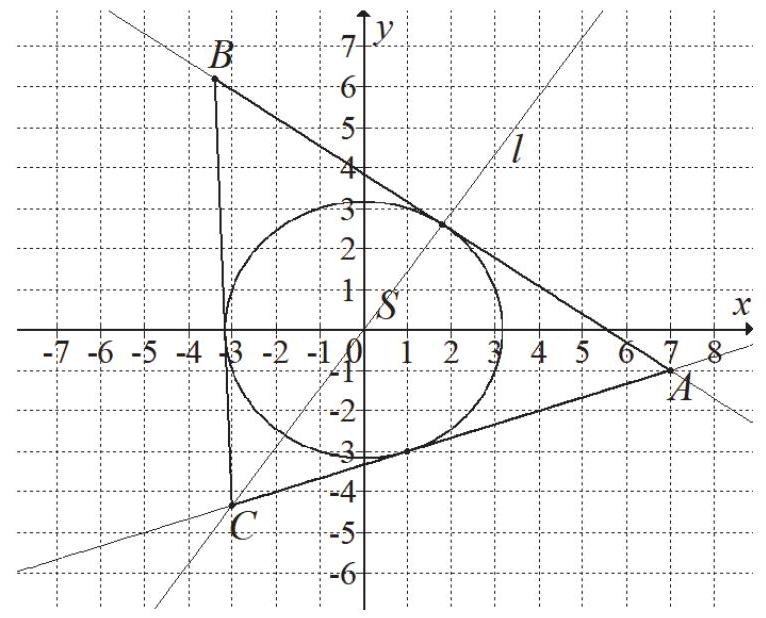
\includegraphics[max width=\textwidth, center]{2025_02_07_a13180f11f288af0ed0dg-24}

Proste $A C$ i $A B$ przechodzą przez punkt $A=(7,-1)$, żadna z nich nie jest prostopadła do osi\\
$O x$ układu współrzędnych, więc mają równania postaci

$$
\begin{gathered}
y=a(x-7)-1, \\
a x-y-7 a-1=0 .
\end{gathered}
$$

Obie te proste są styczne do okręgu, zatem ich odległości od środka okręgu są równe promieniowi okręgu. Stąd otrzymujemy równanie

$$
\begin{gathered}
\frac{|-7 a-1|}{\sqrt{a^{2}+1}}=\sqrt{10}, \\
(-7 a-1)^{2}=10\left(a^{2}+1\right), \\
49 a^{2}+14 a+1=10 a^{2}+10 \\
39 a^{2}+14 a-9=0 \\
a=\frac{-14-40}{78}=-\frac{9}{13} \text { lub } a=\frac{-14+40}{78}=\frac{1}{3} .
\end{gathered}
$$

Szukane styczne mają więc równania: $y=-\frac{9}{13} x+\frac{50}{13}, y=\frac{1}{3} x-\frac{10}{3}$. Tylko druga $z$ tych prostych przechodzi przez trzecią ćwiartkę układu współrzędnych, więc prosta $A C$ ma równanie $y=\frac{1}{3} x-\frac{10}{3}$, a prosta $A B$ ma równanie $y=-\frac{9}{13} x+\frac{50}{13}$.

Trójkąt $A B C$ jest równoramienny, a jego ramionami są boki $A C$ i $B C$. Zatem wierzchołek $C$ leży na przecięciu prostej $A C$ i symetralnej $l$ boku $A B$. Prosta $l$ jest prostopadła do prostej $A B$ i przechodzi przez punkt $S=(0,0)$. Zatem współczynnik kierunkowy prostej $l$ jest równy $a_{l}=\frac{13}{9}$. Stąd $l$ ma równanie postaci

$$
y=\frac{13}{9} x .
$$

Współrzędne wierzchołka $C$ obliczymy, rozwiązując układ równań

$$
y=\frac{1}{3} x-\frac{10}{3} \text { i } y=\frac{13}{9} x .
$$

Stąd otrzymujemy równanie

$$
\begin{gathered}
\frac{1}{3} x-\frac{10}{3}=\frac{13}{9} x, \\
\frac{10}{9} x=-\frac{30}{9} \\
x=-3,
\end{gathered}
$$

więc $y=\frac{13}{9} \cdot(-3)=-\frac{13}{3}$, czyli $C=\left(-3,-\frac{13}{3}\right)$.\\
Obliczamy współrzędne punktu $D$ styczności prostej $A B$ z danym okręgiem. Jest to punkt przecięcia prostej $l$ z prostą $A B$. Wystarczy więc rozwiązać układ równań

$$
y=-\frac{9}{13} x+\frac{50}{13} \text { i } y=\frac{13}{9} x .
$$

Stąd otrzymujemy równanie

$$
\begin{gathered}
-\frac{9}{13} x+\frac{50}{13}=\frac{13}{9} x, \\
\frac{250}{117} x=\frac{50}{13} \\
x=\frac{9}{5},
\end{gathered}
$$

więc $y=\frac{13}{9} \cdot \frac{9}{5}=\frac{13}{5}$, czyli $D=\left(\frac{9}{5}, \frac{13}{5}\right)$.\\
Punkt $D$ jest środkiem odcinka $A B$, więc

$$
D=\left(\frac{7+x_{B}}{2}, \frac{-1+y_{B}}{2}\right) .
$$

Zatem

$$
\begin{gathered}
\frac{7+x_{B}}{2}=\frac{9}{5} \text { i } \frac{-1+y_{B}}{2}=\frac{13}{5}, \\
x_{B}=-\frac{17}{5} \text { i } y_{B}=\frac{31}{5} .
\end{gathered}
$$

Zatem $B=\left(-\frac{17}{5}, \frac{31}{5}\right)$.

\section*{II sposób - syntetycznie - długości odcinków CE i CS}
\begin{center}
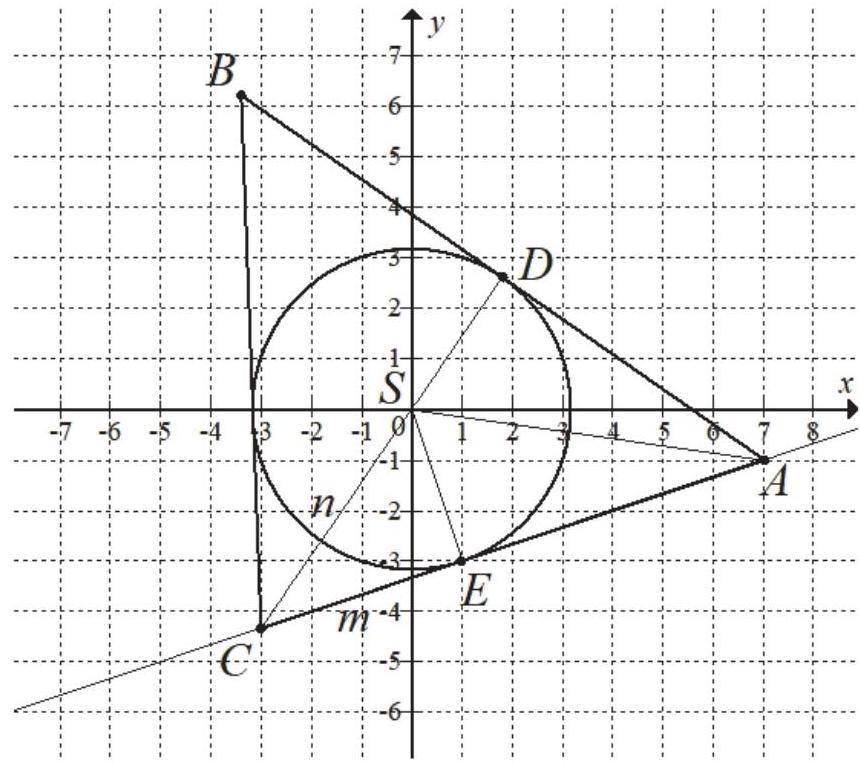
\includegraphics[max width=\textwidth]{2025_02_07_a13180f11f288af0ed0dg-26}
\end{center}

Promień okrę̨u jest równy $r=\sqrt{10}$. Długość odcinka $S A$ jest równa

$$
|S A|=\sqrt{7^{2}+(-1)^{2}}=\sqrt{50}=5 \sqrt{2} .
$$

Z twierdzenia Pitagorasa dla trójkąta $A S E$ otrzymujemy

$$
\begin{gathered}
|S A|^{2}=|S E|^{2}+|E A|^{2}, \\
50=10+E A^{2}, \\
|E A|^{2}=40, \\
|E A|=\sqrt{40}=2 \sqrt{10} .
\end{gathered}
$$

Z twierdzenia o odcinkach stycznych otrzymujemy $|D A|=|E A|=2 \sqrt{10}$.\\
Trójkąty $C E S$ i $C D A$ są podobne, gdyż oba są prostokątne i mają wspólny kąt ostry przy wierzchołku $C$. Stąd wynika

$$
\begin{gathered}
\frac{|C E|}{|S E|}=\frac{|C D|}{|D A|} \text { oraz } \frac{|C S|}{|S E|}=\frac{|C A|}{|D A|}, \\
\frac{m}{\sqrt{10}}=\frac{n+\sqrt{10}}{2 \sqrt{10}} \text { oraz } \frac{n}{\sqrt{10}}=\frac{m+2 \sqrt{10}}{2 \sqrt{10}}, \\
2 m=n+\sqrt{10} \text { oraz } 2 n=m+\sqrt{10}, \\
n=2 m-\sqrt{10} \text { oraz } 2(2 m-\sqrt{10})=m+\sqrt{10} .
\end{gathered}
$$

Stąd

$$
\begin{gathered}
4 m-2 \sqrt{10}=m+\sqrt{10}, \\
m=\frac{4}{3} \sqrt{10}, \text { więc } n=2 \cdot \frac{4}{3} \sqrt{10}-\sqrt{10}=\frac{5}{3} \sqrt{10} .
\end{gathered}
$$

\section*{Uwaga}
Długości $m$ i $n$ możemy też obliczyć korzystając z twierdzenia Pitagorasa dla trójkątów $A C D$ i CSE. Otrzymujemy wtedy

$$
|C A|^{2}=|C D|^{2}+|D A|^{2} \text { oraz }|C S|^{2}=|C E|^{2}+|S E|^{2},
$$

$$
\begin{gathered}
(m+2 \sqrt{10})^{2}=(n+\sqrt{10})^{2}+(2 \sqrt{10})^{2} \text { oraz } n^{2}=m^{2}+(\sqrt{10})^{2}, \\
m^{2}+4 m \sqrt{10}+40=n^{2}+2 n \sqrt{10}+10+40 \text { oraz } n^{2}=m^{2}+10, \\
4 m \sqrt{10}=2 n \sqrt{10}+20 \text { oraz } n^{2}=m^{2}+10, \\
2 m-\sqrt{10}=n \text { oraz }(2 m-\sqrt{10})^{2}=m^{2}+10, \\
2 m-\sqrt{10}=n \text { oraz } 4 m^{2}-4 m \sqrt{10}+10=m^{2}+10, \\
2 m-\sqrt{10}=n \text { oraz } m=\frac{4}{3} \sqrt{10}, \\
n=\frac{5}{3} \sqrt{10} \text { oraz } m=\frac{4}{3} \sqrt{10} .
\end{gathered}
$$

Zatem długość ramienia $A C$ trójkąta $A B C$ jest równa

$$
|A C|=|C E|+|E A|=m+2 \sqrt{10}=\frac{4}{3} \sqrt{10}+2 \sqrt{10}=\frac{10}{3} \sqrt{10} .
$$

Niech $C=(x, y)$. Ponieważ $|A C|=\frac{10}{3} \sqrt{10}$ i $|C S|=\frac{5}{3} \sqrt{10}$, więc

$$
\begin{gathered}
|A C|^{2}=\frac{1000}{9} \text { i }|C S|^{2}=\frac{250}{9}, \\
(x-7)^{2}+(y+1)^{2}=\frac{1000}{9} \text { i } x^{2}+y^{2}=\frac{250}{9} .
\end{gathered}
$$

Pierwsze równanie możemy zapisać w postaci

$$
x^{2}+y^{2}-14 x+2 y+50=\frac{1000}{9} .
$$

Stąd i z drugiego równania otrzymujemy

$$
\begin{gathered}
\frac{250}{9}-14 x+2 y+50=\frac{1000}{9} \\
7 x-y+\frac{50}{3}=0 \\
y=7 x+\frac{150}{9} .
\end{gathered}
$$

Stąd i z pierwszego równania mamy

$$
\begin{gathered}
x^{2}+\left(7 x+\frac{50}{3}\right)^{2}=\frac{250}{9}, \\
x^{2}+49 x^{2}+\frac{700}{3} x+\frac{2500}{9}-\frac{250}{9}=0, \\
50 x^{2}+\frac{700}{3} x+\frac{2250}{9}=0, \\
x^{2}+\frac{14}{3} x+5=0, \\
3 x^{2}+14 x+15=0, \\
3 x^{2}+9 x+5 x+15=0, \\
3 x(x+3) x+5(x+3)=0, \\
(x+3)(3 x+5)=0, \\
x=-3 \text { lub } x=-\frac{5}{3} .
\end{gathered}
$$

Gdy $x=-3$, to $y=7 \cdot(-3)+\frac{50}{3}=-\frac{13}{3}$, a gdy $x=-\frac{5}{3}$, to $y=7 \cdot\left(-\frac{5}{3}\right)+\frac{50}{3}=5$.\\
Ponieważ obie współrzędne punktu $C$ są ujemne, więc $C=\left(-3,-\frac{13}{3}\right)$.

Niech $B=(x, y)$. Ponieważ $|B C|=|A C|=\frac{10}{3} \sqrt{10}$ i $|A B|=2 \cdot 2 \sqrt{10}=4 \sqrt{10}$, więc

$$
\begin{gathered}
|B C|^{2}=\frac{1000}{9} \text { i }|A B|^{2}=160 \\
(-3-x)^{2}+\left(-\frac{13}{3}-y\right)^{2}=\frac{1000}{9} \text { i }(x-7)^{2}+(y+1)^{2}=160 \\
x^{2}+y^{2}+6 x+\frac{26}{3} y-\frac{250}{3}=0 \text { i } x^{2}+y^{2}-14 x+2 y-110=0
\end{gathered}
$$

Stąd

$$
\begin{gathered}
x+\frac{1}{3} y+\frac{4}{3}=0 \text { i } x^{2}+y^{2}-14 x+2 y-110=0 \\
y=-3 x-4 \text { i } x^{2}+(-3 x-4)^{2}-14 x+2(-3 x-4)-110=0
\end{gathered}
$$

Drugie równanie możemy zapisać w postaci

$$
\begin{gathered}
10 x^{2}+4 x-102=0, \\
5 x^{2}+2 x-51=0 \\
\Delta=2^{2}-4 \cdot 5 \cdot(-51)=1024, \sqrt{\Delta}=32, \\
x=\frac{-2-32}{10}=-\frac{17}{5} \text { lub } x=\frac{-2+32}{10}=3,
\end{gathered}
$$

Gdy $x=-\frac{17}{5}$, to $y=-3 \cdot\left(-\frac{17}{5}\right)-4=\frac{31}{5}$, a gdy $x=3$, to $y=-3 \cdot 3-4=-13$.\\
Ponieważ punkt $B$ nie leży w czwartej ćwiartce układu wspórrzędnych, więc $B=\left(-\frac{17}{5}, \frac{31}{5}\right)$.

\section*{Schemat punktowania}
\section*{Rozwiązanie, w którym postęp jest niewielki, ale konieczny na drodze do pełnego rozwiązania zadania}
Zdający:\\
a) obliczy długości odcinków stycznych poprowadzonych z punktu $A$ :

$$
|A D|=|A E|=2 \sqrt{10}
$$

albo\\
b) obliczy współrzędne środka $M$ odcinka $A S$ oraz długość odcinka $A S$,\\
gdzie $S=(0,0): M=\left(\frac{7}{2},-\frac{1}{2}\right),|A S|=5 \sqrt{2}$,\\
albo\\
c) obliczy sinus kąta $S A E: \sin \alpha=\frac{\sqrt{5}}{5}$,\\
albo\\
d) zapisze równanie pęku prostych przechodzących przez punkt $A: y=a x-7 a-1$, albo\\
e) zapisze, że trójkąt $A D C$ jest podobny do trójkąta $S E C$,\\
f) obliczy długość tylko jednego z odcinków $A D$ lub $A E:|A D|=|A E|=2 \sqrt{10}$ oraz zapisze tę długość w zależności od współrzędnych punktu $D$ (lub $E$ ) lub obliczy tangens kąta $S A E$ lub $S A D: \operatorname{tg} \alpha=\frac{1}{2}$\\
i na tym zakończy lub dalej popełnia błędy.

\section*{Rozwiązanie, w którym istotny postęp}
Zdający:\\
A) obliczy $|A D|=2 \sqrt{10}$ oraz zapisze układ równań $\left\{\begin{array}{l}(x-7)^{2}+(y+1)^{2}=40 \\ x^{2}+y^{2}=10\end{array}\right.$\\
albo\\
B) obliczy $|A D|=|A E|=2 \sqrt{10}$ oraz zapisze układ równań z niewiadomymi $m=|C E|$ i $n=|C S|:$

\begin{itemize}
  \item $\frac{m}{\sqrt{10}}=\frac{n+\sqrt{10}}{2 \sqrt{10}} \mathrm{i} \frac{n}{\sqrt{10}}=\frac{m+\sqrt{10}}{2 \sqrt{10}}$
  \item $(m+2 \sqrt{10})^{2}=(n+\sqrt{10})^{2}+(2 \sqrt{10})^{2}$ i $n^{2}=m^{2}+(\sqrt{10})^{2}$\\
albo\\
C) obliczy $|A D|=2 \sqrt{10}$, obliczy tangens kąta $S A E: \operatorname{tg} \alpha=\frac{1}{2}$ oraz obliczy współczynnik kierunkowy prostej $A S \quad\left(a_{A S}=-\frac{1}{7}\right)$\\
albo\\
D) obliczy współrzędne środka $M=\left(\frac{7}{2},-\frac{1}{2}\right)$, długość odcinka $|A S|=5 \sqrt{2}$ oraz zapisze układ równań $\left\{\begin{array}{l}\left(x-\frac{7}{2}\right)^{2}+\left(y+\frac{1}{2}\right)^{2}=\frac{25}{2} \\ x^{2}+y^{2}=10\end{array}\right.$\\
albo\\
E) obliczy sinus kąta $S A E: \sin \alpha=\frac{\sqrt{5}}{5}$, tangens tego kąta: $\operatorname{tg} \alpha=\frac{1}{2}$ oraz współczynnik kierunkowy prostej $A S\left(a_{A S}=-\frac{1}{7}\right)$\\
albo\\
F) zapisze równanie pęku prostych przechodzących przez punkt $A$ : $y=a x-7 a-1$ oraz równanie z niewiadomą $a: \frac{|-7 a-1|}{\sqrt{a^{2}+1}}=\sqrt{10}$\\
albo\\
G) zapisze równanie pęku prostych przechodzących przez punkt $A$ : $y=a x-7 a-1$ oraz układu równań $x^{2}+y^{2}=10$ i $y=a x-7 a-1$ wraz z warunkiem istnienia jednego rozwiązania tego układu\\
i na tym zakończy lub dalej popełnia błędy.\\
Pokonanie zasadniczych trudności zadania 3 p.\\
Zdający:\\
I obliczy współrzędne punktów styczności $D$ i $E: D=\left(\frac{9}{5}, \frac{13}{5}\right), E=(1,-3)$\\
albo\\
II zapisze równania prostych $A C$ i $A B: y=\frac{1}{3} x-\frac{10}{3}, y=-\frac{9}{13} x+\frac{50}{13}$\\
albo\\
III obliczy długości odcinków $C E$ i $C S: m=|C E|=\frac{4}{3} \sqrt{10}, \quad n=|C S|=\frac{4}{3} \sqrt{10}$ i na tym zakończy lub dalej popełnia błędy.
\end{itemize}

\section*{Zdający}
\begin{itemize}
  \item obliczy współrzędne wierzchołka $B: B=\left(-\frac{17}{5}, \frac{31}{5}\right)$\\
albo
  \item obliczy współrzędne wierzchołka $C$ : $C=\left(-3,-\frac{13}{3}\right)$
\end{itemize}

\section*{Uwaga}
Jeżeli zdający

\begin{itemize}
  \item obliczy współrzędne wierzchołka $B: B=\left(-\frac{17}{5}, \frac{31}{5}\right)$ oraz zapisze układ równań z niewiadomymi $x, y$-współrzędnymi wierzchołka $C$, np.: $x-3 y-10=0$\\
i $13 x-9 y=0$\\
albo
  \item obliczy współrzędne wierzchołka $C$ : $C=\left(-3,-\frac{13}{3}\right)$ oraz zapisze układ równań z niewiadomymi $x, y$-współrłzędnymi wierzchołka $B$, np.: $\frac{x+7}{2}=\frac{9}{5} \mathrm{i} \frac{y-1}{2}=\frac{13}{5}$\\
albo
  \item obliczy współrzędne obu wierzchołków $B$ i $C$, popełniając w trakcie rozwiązania błędy rachunkowe\\
to otrzymuje 5 punktów.\\
Rozwiązanie pełne 6 p.\\
Zdający obliczy współrzędne wierzchołków $B$ i $C: B=\left(-\frac{17}{5}, \frac{31}{5}\right), C=\left(-3,-\frac{13}{3}\right)$.
\end{itemize}

\section*{Uwagi}
\begin{enumerate}
  \item Jeżeli zdający pominie informację o ujemnych współrzędnych punktu $C$ i tym samym zamieni miejscami proste $A C$ i $A B$, to może otrzymać 5 punktów za całe rozwiązanie, o ile nie popełni innych błędów.
  \item Jeżeli zdający błędnie przyjmuje, że podstawą trójkąta jest inny bok niż $A B$, to może otrzymać co najwyżej 5 punktów.
  \item Jeżeli zdający realizuje strategię rozwiązania i popełnia jedynie błędy rachunkowe, to może otrzymać 5 punktów, o ile popełnione błędy nie ułatwiają rozwiązania zadania na żadnym etapie.
  \item Jeżeli zdający zapisze dwa równania $z$ dwiema niewiadomymi, którymi są współrzędne punktu $B$ lub $C$, to otrzymuje 2 punkty.
  \item Jeżeli zdający odczytuje z rysunku współrzędne punktu $E$, a następnie wyznacza równanie stycznej $A E$ i na tym poprzestaje, to może otrzymać $\mathbf{1}$ punkt.
\end{enumerate}

Zadanie 15. (0-7)

\begin{center}
\begin{tabular}{|l|l|}
\hline
 & \begin{tabular}{l}
7. Planimetria. Zdający znajduje związki miarowe \\
w figurach płaskich z zastosowaniem twierdzenia \\
III. Modelowanie \\
matematyczne. \\
\end{tabular} \\
\begin{tabular}{l}
11. Rachunek róż̇niczkowy. Zdający stosuje pochodne \\
do rozwiązywania zagadnień optymalizacyjnych \\
(R11.6). \\
\end{tabular} &  \\
\hline
\end{tabular}
\end{center}

\section*{Przykładowe rozwiązanie}
Przyjmijmy oznaczenia jak na rysunku.\\
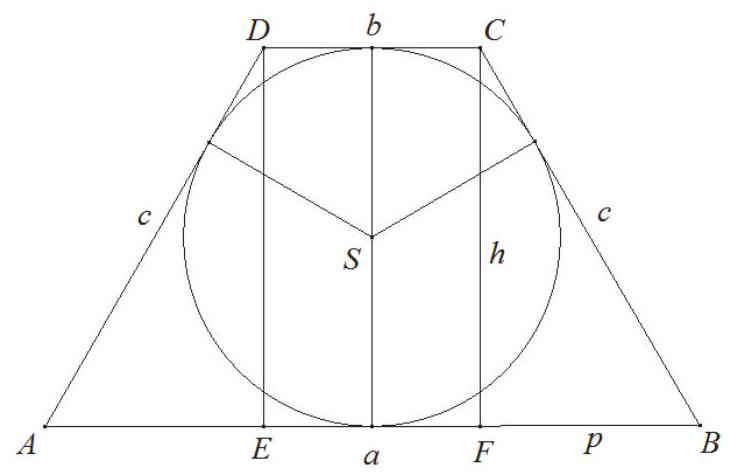
\includegraphics[max width=\textwidth, center]{2025_02_07_a13180f11f288af0ed0dg-31}

Wyznaczmy dziedzinę funkcji $L$. Z warunków zadania wynika, że $a>h$, więc $a>2-a$. Stąd $a>1$. Jeśli $a=1$, to czworokąt jest kwadratem. Ponadto $a<2$. Jeśli $a=2$, to $h=0$ i zamiast trapezu mamy do czynienia z odcinkiem o długości 2.\\
Rozważany trapez istnieje jedynie dla $a \in(1,2)$.\\
Z warunków zadania otrzymujemy

$$
a+h=2, \operatorname{skąd} h=2-a \text {. }
$$

Ponieważ w trapez można wpisać okrąg, więc

$$
a+b=2 c .
$$

Obwód $L$ trapezu jest więc równy

$$
L=a+b+2 c=2(a+b) .
$$

Trapez jest równoramienny, więc odcinki $A E$ i $F B$ mają tę samą długość równą

$$
p=\frac{a-b}{2} .
$$

Z twierdzenia Pitagorasa dla trójkąta $B C F$ otrzymujemy

$$
\begin{aligned}
p^{2}+h^{2} & =c^{2}, \\
\left(\frac{a-b}{2}\right)^{2}+h^{2} & =\left(\frac{a+b}{2}\right)^{2}, \\
\frac{a^{2}}{4}-\frac{a b}{2}+\frac{b^{2}}{4}+h^{2} & =\frac{a^{2}}{4}+\frac{a b}{2}+\frac{b^{2}}{4}, \\
h^{2} & =a b, \\
(2-a)^{2} & =a b,
\end{aligned}
$$

$$
b=\frac{(2-a)^{2}}{a}=\frac{a^{2}-4 a+4}{a} .
$$

Zatem

$$
L=a+b+2 c=2(a+b)=2\left(a+\frac{a^{2}-4 a+4}{a}\right)=2 \cdot \frac{2 a^{2}-4 a+4}{a},
$$

czyli

$$
L(a)=\frac{4 a^{2}-8 a+8}{a} \text { dla } a \in(1,2) .
$$

Pochodna funkcji $L$ jest równa\\
$L^{\prime}(a)=\frac{(8 a-8) \cdot a-\left(4 a^{2}-8 a+8\right) \cdot 1}{a^{2}}=\frac{4 a^{2}-8}{a^{2}}=\frac{4(a-\sqrt{2})(a+\sqrt{2})}{a^{2}}$ dla $a \in(1,2)$.\\
Ponieważ dla każdego $a \in(1,2)$ prawdziwa jest nierówność $\frac{4(a+\sqrt{2})}{a^{2}}>0$, więc\\
$L^{\prime}(a)=0 \Leftrightarrow a-\sqrt{2}=0 \wedge a \in(1,2) \Leftrightarrow a=\sqrt{2}$,\\
$L^{\prime}(a)>0 \Leftrightarrow a-\sqrt{2}>0 \wedge a \in(1,2) \Leftrightarrow a \in(\sqrt{2}, 2)$,\\
$L^{\prime}(a)<0 \Leftrightarrow a-\sqrt{2}<0 \wedge a \in(1,2) \Leftrightarrow a \in(1, \sqrt{2})$.\\
Oznacza to, że w przedziale $(1, \sqrt{2}\rangle$ funkcja $L$ jest malejąca, w przedziale $\langle\sqrt{2}, 2)$ jest rosnąca, a w punkcie $a=\sqrt{2}$ osiąga minimum lokalne, które jest zarazem jej najmniejszą wartością.\\
Tangens kąta ostrego trapezu o najmniejszym obwodzie jest równy

$$
\operatorname{tg} \Varangle A B C=\frac{h}{p}=\frac{2-a}{\frac{a-b}{2}}=\frac{2(2-a)}{a-\frac{a^{2}-4 a+4}{a}}=\frac{a(a-2)}{2(1-a)},
$$

więc dla $a=\sqrt{2}$ wartość tangensa jest równa

$$
\operatorname{tg} \Varangle A B C=\frac{\sqrt{2}(\sqrt{2}-2)}{2(1-\sqrt{2})}=\frac{2-2 \sqrt{2}}{2-2 \sqrt{2}}=1,
$$

co oznacza, że $\Varangle A B C=45^{\circ}$.

\section*{Schemat oceniania}
Rozwiązanie zadania składa się z trzech etapów. Ocenianie II etapu jest niezależne od wyniku uzyskanego za I etap.\\
I. Pierwszy etap, który oceniamy na $\mathbf{3}$ punkty, składa się z trzech części:\\
I.1) wyznaczenie wszystkich wartości $a$, dla których istnieje trapez o podanych własnościach, czyli dziedziny funkcji $L: D_{L}=(1,2)$\\
(Za wyznaczenie dziedziny uznaje się też zapisanie dwóch nierówności: $2-a>0$,

$$
a>2-a) .
$$

I.2) zapisanie poprawnej zależności między wielkościami $a$ i $b$, np.:

$$
\left(\frac{a-b}{2}\right)^{2}+(2-a)^{2}=\left(\frac{a+b}{2}\right)^{2} \text { lub } b=\frac{a^{2}-4 a+4}{a}
$$

I.3) wykazanie, że obwód $L$ trapezu, jako funkcja zmiennej $a$, wyraża się wzorem:

$$
L(a)=\frac{4 a^{2}-8 a+8}{a}
$$

Za poprawne rozwiązanie każdej z części tego etapu zdający otrzymuje $\mathbf{1}$ punkt.\\
II. Drugi etap ( $\mathbf{3}$ punkty) składa się z trzech części:\\
II.1) wyznaczenie pochodnej funkcji $f(a)=\frac{4 a^{2}-8 a+8}{a}$ :

$$
f^{\prime}(a)=\frac{(8 a-8) \cdot a-\left(4 a^{2}-8 a+8\right) \cdot 1}{a^{2}} \text { lub } f^{\prime}(a)=\frac{4 a^{2}-8}{a^{2}}
$$

II.2) obliczenie miejsc zerowych pochodnej funkcji $f: a=-\sqrt{2}$ lub $a=\sqrt{2}$\\
II.3) uzasadnienie (np. badanie monotoniczności funkcji), że funkcja $L$ posiada wartość najmniejszą dla $a=\sqrt{2}$.\\
III. Trzeci etap (1 punkt) - obliczenie tangensa kąta ostrego trapezu o najmniejszym polu: $\operatorname{tg} \Varangle A B C=1$.

\section*{Uwagi}
\begin{enumerate}
  \item Za poprawne uzasadnienie, że funkcja $L$ posiada wartość najmniejszą dla wyznaczonej wartości $a$, przy której pochodna się zeruje można uznać sytuacje, gdy zdający:
\end{enumerate}

\begin{itemize}
  \item opisuje, słownie lub graficznie (np. przy użyciu strzałek), monotoniczność funkcji $L$;
  \item zapisuje, że dla wyznaczonej wartości $a$ funkcja $L$ ma minimum lokalne i jest to jednocześnie jej najmniejsza wartość.\\
Jeżeli zdający nie przedstawi takiego uzasadnienia, to za II etap może otrzymać co najwyżej 2 punkty.
\end{itemize}

\begin{enumerate}
  \setcounter{enumi}{1}
  \item Jeżeli zdający przyjmuje, że dziedziną funkcji $L$ jest przedział $(0,+\infty)$ lub nie wyznaczy tej dziedziny, to nie otrzymuje punktów za realizację części II.3.
  \item Jeżeli zdający przyjmuje, że dziedziną funkcji $L$ jest przedział $(0,2)$ lub zapisze warunki: $2-a>0$ i $a>0$, to może otrzymać 1 punkt za realizację części II.3., o ile uzasadni istnienie najmniejszej wartości funkcji.
  \item Jeżeli zdający przyjmuje, że dziedziną funkcji $L$ jest przedział ( $1,+\infty$ ) lub zapisze warunki: $a>h$ i $h>0$, lub zapisze warunek $a>2-a$, to może otrzymać $\mathbf{1}$ punkt za realizację części II.3., o ile uzasadni istnienie najmniejszej wartości funkcji.
  \item Jeżeli zdający przyjmuje, że dziedziną funkcji $L$ jest przedział $\langle 1,2)$, to za realizację etapu
\end{enumerate}

\section*{I. 1 otrzymuje 1 punkt.}
\begin{enumerate}
  \setcounter{enumi}{5}
  \item Jeżeli zdający w wyniku błędów nie wyznaczy poprawnie długości dłużej podstawy trapezu o najmniejszym obwodzie, ale dla wyznaczonej wartości $a$ obliczy tangens kąta ostrego trapezu, to może otrzymać $\mathbf{1}$ punkt za III etap.
  \item Jeżeli zdający bada inną funkcję zmiennej $a$ niż postaci $g(a)=k \cdot \frac{4 a^{2}-8 a+8}{a}$, gdzie $k \neq 0$, to nie otrzymuje punktów za II i III etap rozwiązania.
  \item Jeżeli z zapisu rozwiązania wynika, że zdający stosuje poprawny wzór na pochodną ilorazu funkcji i dalej popełnia błędy, ale otrzymana w rozwiązaniu pochodna ma dwa różne miejsca zerowe, to zdający może otrzymać w II etapie punkty za konsekwentną realizację części II.2)\\
i II.3). Jeżeli z zapisu rozwiązania nie wynika, że zdający stosuje poprawny wzór na pochodną ilorazu funkcji i zdający popełnia błędy przy obliczaniu pochodnej, ale otrzymuje wzór na pochodną, w którym w liczniku jest wielomian stopnia 2 , a w mianowniku $a^{2}$, to może w II etapie otrzymać jedynie punkt za konsekwentną realizację części II.3.
\end{enumerate}

\end{document}